\documentclass[11pt,oneside]{article}
\usepackage{style-3yp}
\lfoot{Lai Chong}
\let\subsubsubsection\paragraph
\begin{document}

\section{Air Separation}
%\tableofcontents        

\subsection{Introduction} \noindent
This section will briefly discuss the aim of the air separation part of the project, the goals to achieve as well as the two conventional air separation methods used in the industry.
	\subsubsection{Background}  \noindent
    One of the two major inputs to the Haber-Bosch process for the ammonia synthesis part of the energy storage system is a high-purity stream of nitrogen. This section details the method used to process around 265.5 tpd of dry air to produce 202.8 tpd of nitrogen at 99.99\% purity to be further processed in the Haber-Bosch plant downstream, to produce 90,000 tpy of Ammonia.
	\subsubsection{Air Composition} \noindent
    The input to the processing plant is atmospheric air taken at ambient temperature and pressure (at 25$^\circ$C and 1.013 bar). A water filter unit is in place to remove any water content in the input stream before air separation. Details of the dry air composition are as shown in the table \ref{table:air_properties} \citep{hands1986,barron1985,HLT}.
    \begin{table}[ht]
        \singlespacing
	    \centering
	    \caption{Air Composition and Properties}
	    \label{table:air_properties}
        
	    \begin{tabular}{|c|cccc|}
	    \hline
	    Species 	& Molecular Weight	& Mole Fraction & Boiling Point 	& Specific Heat $\tilde{c}_p$ \\
                    & (kg kmol$^{-1}$)    &               & (K)               & (kJ kmol$^{-1}$K$^{-1}$)\\
	    \hline
	    N$_2$		& 28.01				& 78.08\%		& 77.4				& 29.10 \\
	    O$_2$		& 32.00				& 20.95\%		& 90.2				& 29.28 \\
	    Ar			& 39.95				& 0.93\%		& 87.3				& 20.77 \\ 
	    CO$_2$		& 44.01				& 0.03\%		&					& 36.04 \\
	    Other Gases &					& Trace	    	& 					&       \\
	    \hline
	    Air         & 28.96             & 100\%         &                   & 29.08 \\
	    \hline
	    \end{tabular}
    \end{table}
	\subsubsection{Production Methods} \noindent
    Conventional air separation plants adopt either Pressure Swing Adsorption (PSA) or Cryogenic Distillation to separate nitrogen (or oxygen, depending the purpose of the plant) from air. \\
    Both methods have their own distinctive advantages and disadvantages, and a decision  is made based on the following two criteria: production capacity and purity of desired product.  
		\subsubsubsection{Pressure Swing Adsorption}
        Pressure Swing Adsorption makes use of the differences in gas species' properties and their respective affinities for the adsorbent material under pressure to separate from a mixture of gases \citep{linde_PSA}. \\
        An adsorbent bed is used in a PSA column, which preferentially adsorbs nitrogen under pressure and allows other gases to be removed. After separation, adsorbent bed is regenerated by lowering column pressure, thus releasing the adsorbed nitrogen.\\
        The PSA column operates as a batch process, hence as a conventional practice in the industry, two  (or more) columns are ran in an alternating sequence to separate gases continuously.\\
        Capacities of PSA plants can range from small scale of 100 m$^3$/hr at 99.9\% nitrogen purity to large scale of 9000 m$^3$/hr at 97\% nitrogen purity \citep{PRISM}. \\
        As this method does not satisfy the 99.99\% nitrogen purity requirement, more in-depth details of this method is not investigated further.
		\subsubsubsection{Cryogenic Distillation}
        Cryogenic Distillation makes use of the differences in gas species' boiling points and their respective volatilities under cryogenic temperatures to separate from a mixture of gases \citep{linde_cryo}.\\
        Depending on the purity requirements of products, design of one to three distillation columns is used, namely high-pressure column (HPC), low-pressure column (LPC) and argon column (ARC). Input stream of air is filtered and liquefied before entering the system distillation columns, producing high-purity nitrogen from the top of the column and oxygen-rich mixture from the bottom (assuming a two-column design).\\
        Capacities of cryogenic distillation plants can range from small scale of 600 tpd to large scale of 40,000 tpd of nitrogen at very high purity; though the plants' load range are highly inflexible with a low ramp-rate, it is not ideal to turn the unit off and on which poses a problem with varying wind supply. \\
        This method satisfies both production capacity and purity requirements, hence the method is adopted for our plant and the design details are investigated further. And to address the varying wind supply issue, the unit is designed to run continuously.
\subsection{Plant Overview} \noindent
This section includes the overall air separation plant schematic and goes over individual component of the plant. Working equations and design parameters are specified in this section, allowing optimisation and analysis in the next section.
	\subsubsection{Plant Diagram} \noindent
    A diagram of the air separation plant is shown on next page in figure \ref{plant_diagram}, which is an adaption from a cryogenic air separation plant schematic by Linde Engineering \cite{linde_cryo}.
    \begin{sidewaysfigure}[p]
        \centering
	    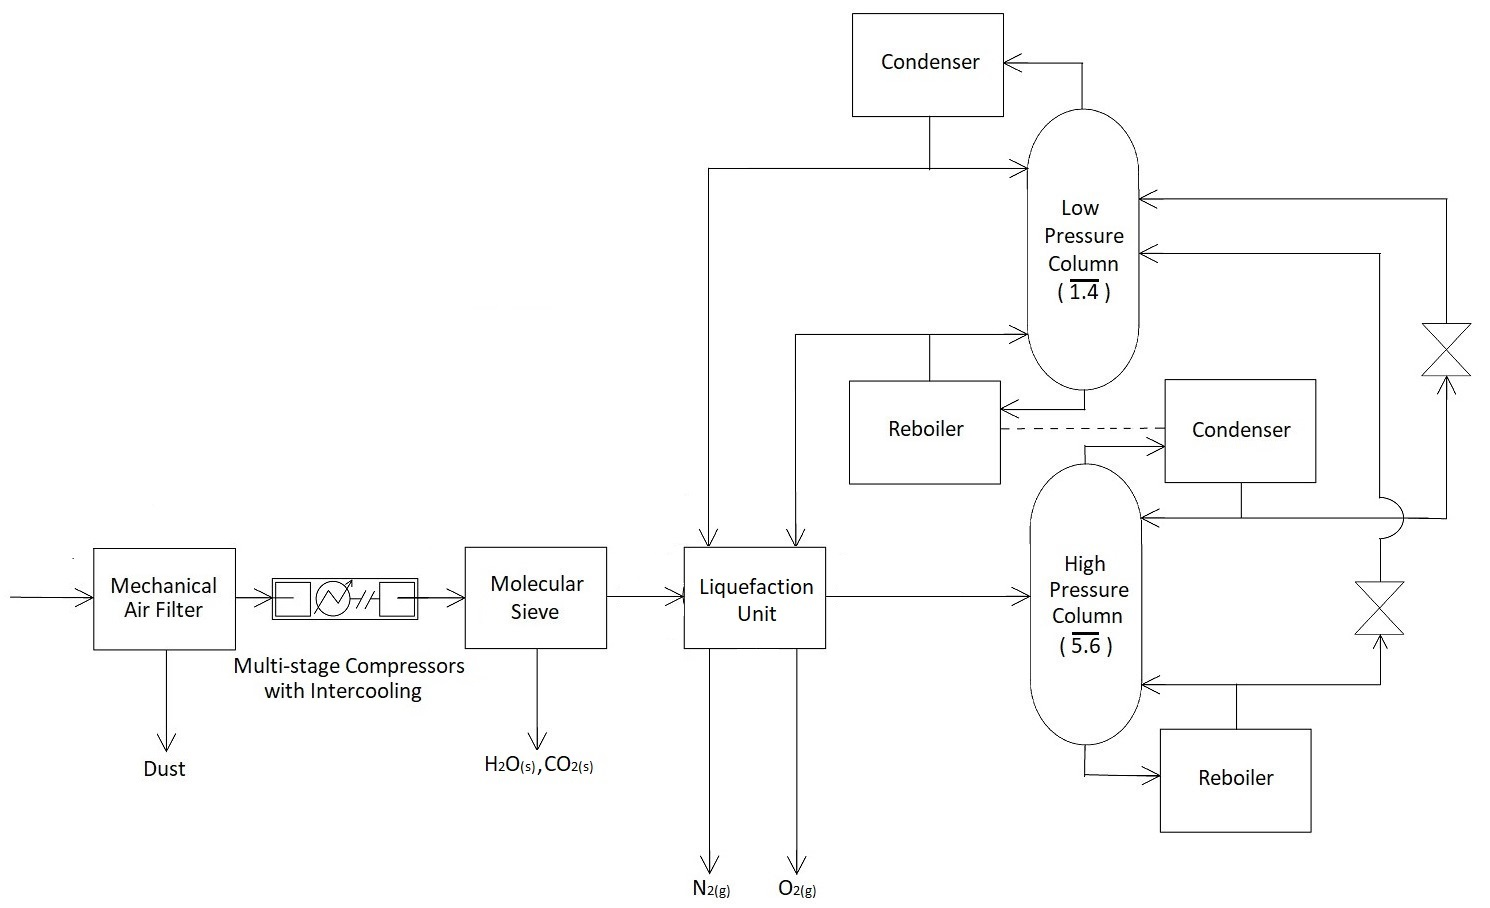
\includegraphics[width=\linewidth]{plant_diagram.jpg}
        \caption{Overall Plant Schematic (adapted from Linde Engineering cryogenic air separation process)}
	    \label{plant_diagram}
    \end{sidewaysfigure}
	\subsubsection{Plant Components} \noindent
    Adapted from a cryogenic air separation plant schematic by Linde Engineering, the plant will contain the following components \citep{linde_cryo}:
    \begin{table}[ht]
        \singlespacing
    	\centering
	    \caption{Cryogenic Plant Components}
	    \label{table:plant_components}

	    \begin{tabular}{|l|l|}
	    \hline
	    Component						& Purpose \\        \hline
	    Mechanical air filter 			& Dust removal \\
	    Molecular sieve					& H$_2$O and CO$_2$ removal \\
	    Multi-stage compressors with intercoolers & Bring inlet to optimum temperature and pressure\\
	    Throttle (or expansion turbine)	& Lower pressure to transition between HPC and LPC\\
	    High-pressure column			& First-stage distillation \\
	    Low-pressure column				& Second-stage purification \\
	    Reboiler and condenser units	& Regulate column conditions\\
	    Heat exchangers					& Using the cold product to cool inlet stream \\  \hline
	    \end{tabular}
    \end{table}
		\subsubsubsection{Pre-Processing Filtering}
        Before inlet air stream can enter the first distillation column for separation, it has to be processed to remove impurities that may adversely affect the performance of the plant, namely water vapour and carbon dioxide. \\
        A mechanical air filter is first used to remove solid air particulates by means of a woven fibrous membrane in a cylindrical cartridge (up to 0.5 \textmu m). Air flows from outside in, accumulating dust on the exterior of the cylinder, which can be blown off by a reverse pulse of compressed air \citep{airfilter}.\\
        Water vapour can condense into ice in the cryogenic chambers, the build-up can cause blockage in the trays of distillation column; whilst carbon dioxide can poison the catalyst in Haber-Bosch process downstream. Hence both species are removed via the use of a molecular sieve, which uses microporous adsorbents like zeolite (up to 2 nm) and operates in a similar manner as PSA \citep{white2017}.
        \subsubsubsection{Multi-stage Compressors with Intercoolers}
        In between the air filter and the molecular sieve, a multi-stage compressor will be used compress filtered inlet gas stream from 1.01 bar (i.e. atmospheric) to 5.6 bar. As the compression process is modelled to be adiabatic, temperature of the inlet stream will rise with compression, hence intercoolers are used to ensure maximum temperature in between compression is capped at 400 K to ensure minimal heat transfer and high compressor efficiency. \\
        After the first compression, hot compressed gas is cooled to ambient temperature (298 K) using water as a coolant before subjected to further compression. This process is repeated if multiple stages of compression is required.\\
        By using ideal gas law ($pv=RT$) and assuming polytropic process ($pv^\gamma=constant$), compression pressure ratio can be defined by equation \ref{eq:rp}:
        \begin{equation}
            r_p = \frac{p_{out}}{p_{in}} = \left(\frac{T_{out}}{T_{in}}\right)^\frac{\gamma}{\gamma-1}
            \label{eq:rp}
        \end{equation}
        It follows that single-stage work input can be defined by equation \ref{eq:work}:
        \begin{equation}
            W_{in}=\frac{\gamma}{\gamma-1}\dot{m}c_pT_{in}\left(r_p^{\frac{\gamma-1}{\gamma}}-1\right)\cdot\frac{1}{\eta_{mech}}
            \label{eq:work}
        \end{equation}
        where $\dot{m}$ is inlet stream mass flow rate (= 265.5 tpd of dry air, or 3.07 kgs$^{-1}$), $c_p$ is the specific heat capacity of air mixture, $T_{in}$ is the inlet temperature, {\textgamma} is the Poisson constant (= 1.4 for adiabatic process) and ${\eta}_{mech}$ is the mechanical efficiency of compressor (assuming 90\% efficient).\\
        \\
        Specific heat capacity of air mixture at constant pressure changes with varying temperature, from 1.01 kJ kmol$^{-1}$K$^{-1}$ at 298K to 1.07 kJ kmol$^{-1}$K$^{-1}$ at 400K (at constant pressure of 5 bar) \citep{engtoolbox_cp}. As there is only a small increase in value, 1.01 kJ kmol$^{-1}$K$^{-1}$ is used to simplify calculations. \\  
        Abiding by the temperature cap, first stage compresses inlet air stream from 1 bar to 2.80 bar, with predicted compressor work of 1229 kW. Second stage compresses air stream from 2.80 bar to 5.60 bar, with predicted compressor work of 787 kW. This gives a total of 2016 kW of compressor work before liquefaction.
        \subsubsubsection{Liquefaction Unit}
        Inlet air stream has to be cooled and fully liquefied before feeding into the HPC for separation. But with the low boiling point of species, it is difficult to find a refrigerant that can be used to achieve the goal. \\
        Hence a modified Linde-Hampson liquefaction cycle is used as shown in figure \ref{labelled_liquefier_diagram} \citep{barron1985}. \\
        \begin{figure}[H]
            \centering
            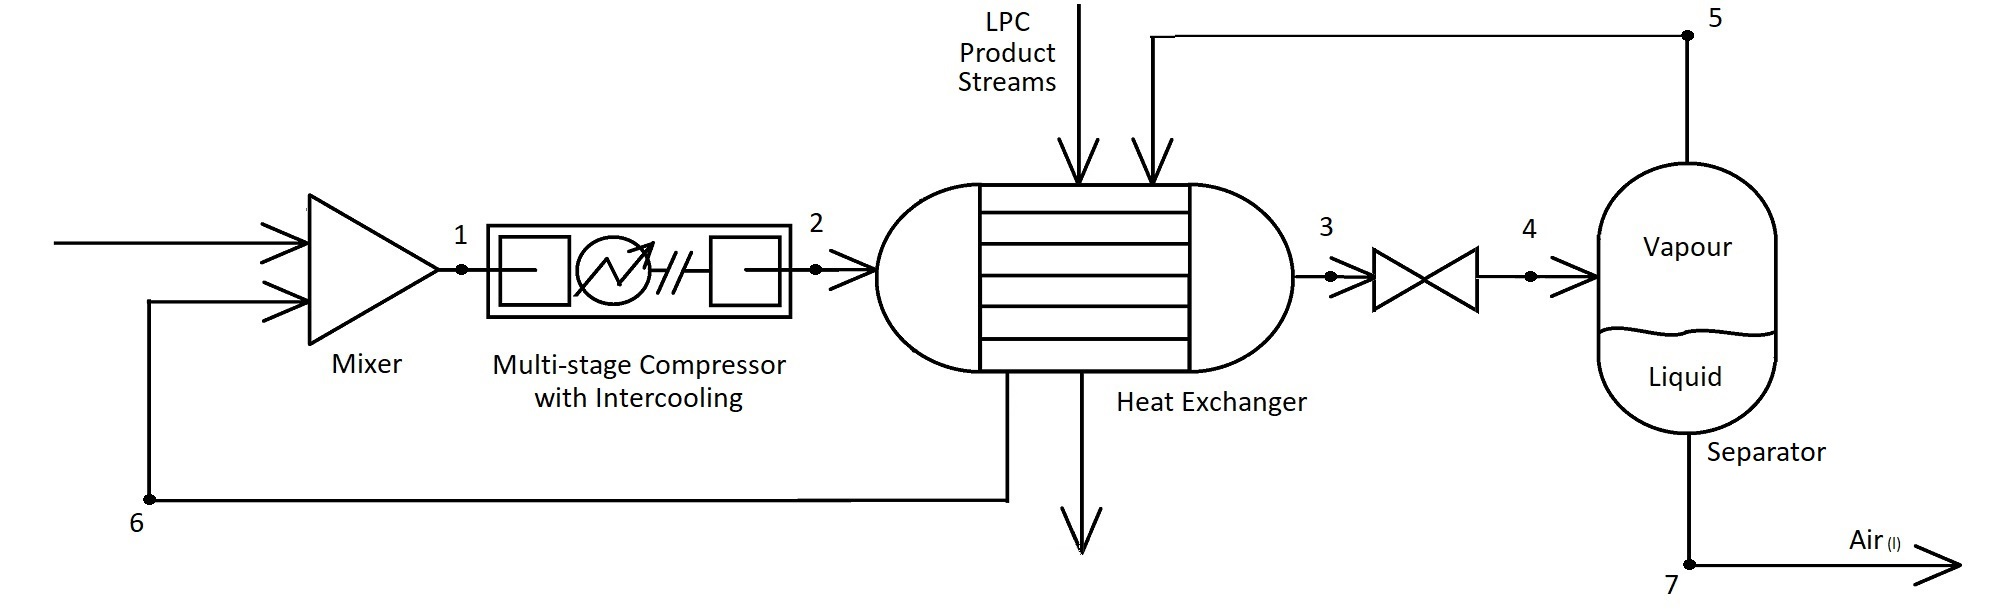
\includegraphics[scale=0.4]{labelled_liquefier_diagram.jpg}
            \caption{Modified Linde-Hampson Liquefaction Cycle}
            \label{labelled_liquefier_diagram}
        \end{figure}
        \noindent Inlet air stream is compressed from 5.60 bar to 50 bar in another multi-stage compressor with intercooling, but for simplicity this compression process will be modelled as isothermal compression (state 1 $\rightarrow$ 2). After compression, inlet air stream will be cooled using both the vapour stream from the separator and the two product streams from LPC (state 2 $\rightarrow$ 3, with reference to figure \ref{plant_diagram}) in a series of heat exchangers. This will cool the inlet air stream to cryogenic temperature at 50 bar, which will then be put through a throttle for isentropic expansion to 5.6 bar (state 3 $\rightarrow$ 4). Inlet air stream is now in saturated liquid-vapour state and can be separated by state in the separator. Liquid stream (state 7) is extracted from the bottom of the separator and can now enter the HPC for first-stage separation; whilst vapour stream (state 5) is recycled, cold is extracted (state 5 $\rightarrow$ 6) and mixed in with incoming inlet air stream to be liquefied again. \\
        This process is depicted in a temperature-entropy diagram of air as shown in figure \ref{liquefier_T-S_diagram}. Note that each node correspond to their respective streams in the liquefaction unit diagram in figure \ref{labelled_liquefier_diagram}. \\
        \begin{figure}[H]
            \centering
            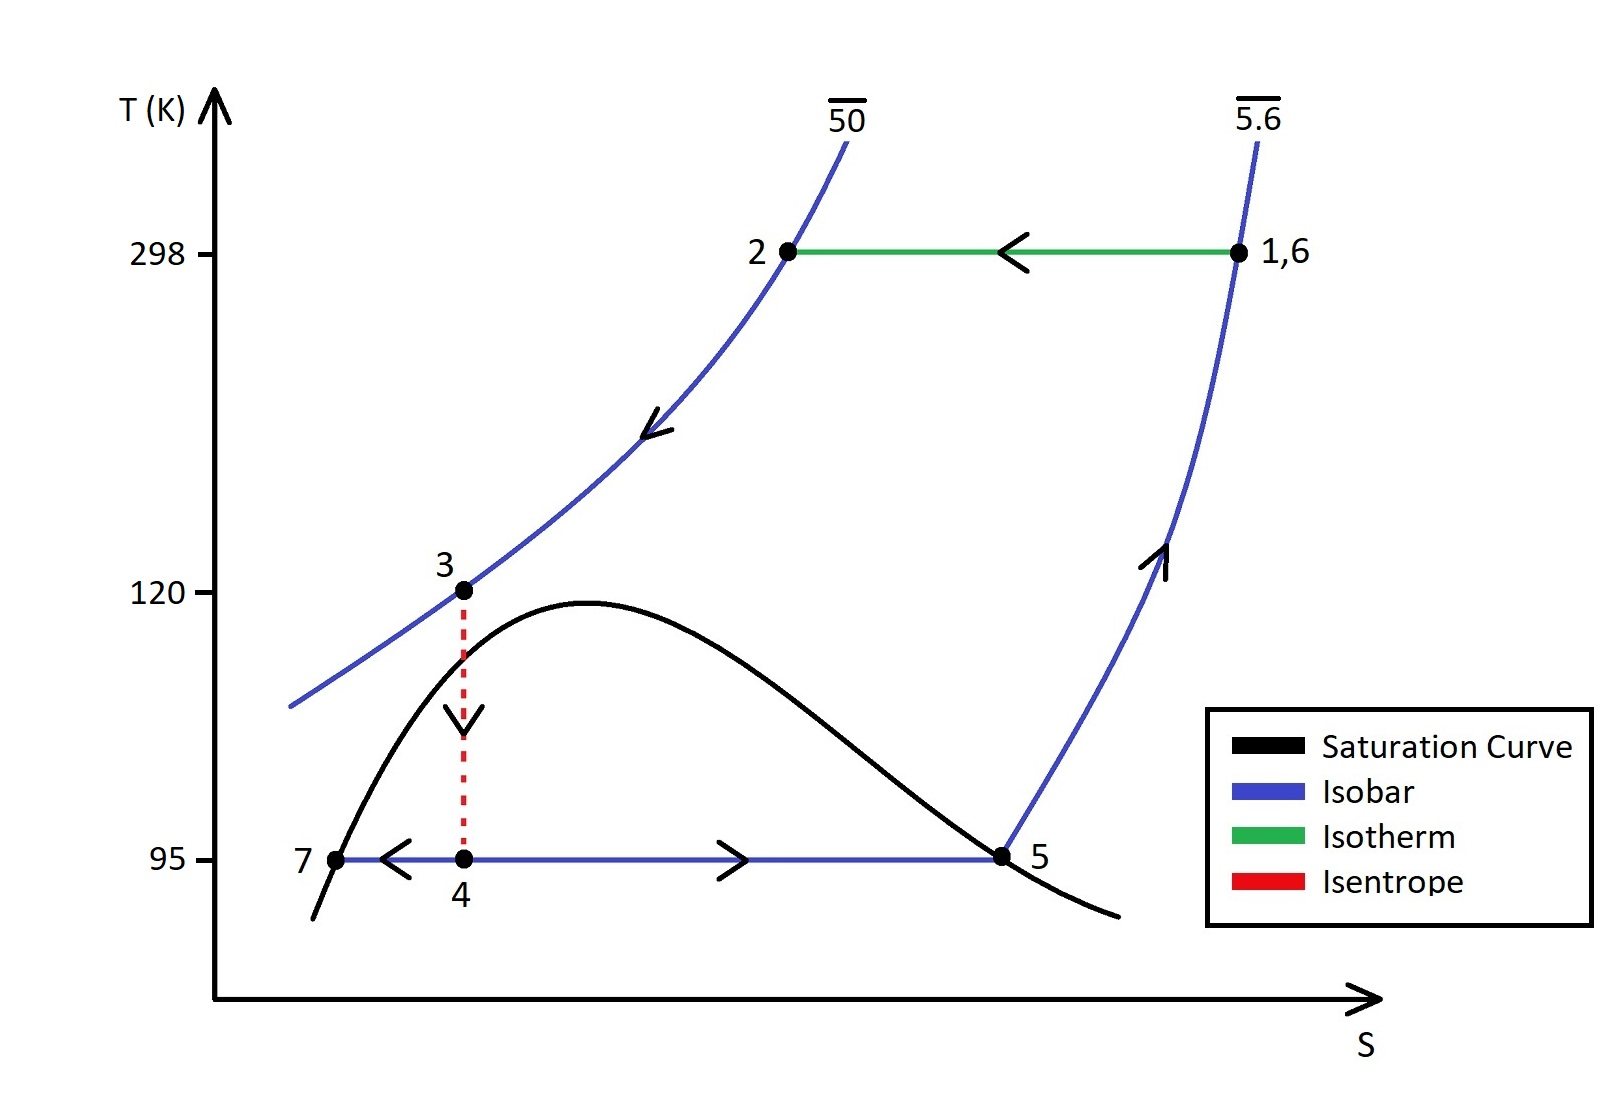
\includegraphics[scale=0.3]{liquefier_T-S_diagram.jpg}
            \caption{Temperature-Entropy Diagram of Linde-Hampson Liquefaction Cycle}
            \label{liquefier_T-S_diagram}
        \end{figure}
        \noindent Most temperature and pressure conditions are already well-defined, except the temperature at state 3. If the temperature is increased at state 3, less heat exchange is required between the cold and hot streams hence a smaller heat exchanger can be used (i.e. reduction in capital cost); the downsides of this decision are losing more work at the throttle as well as smaller fraction of the stream is liquefied thus requiring a larger recycle stream (i.e. lower efficiency). For simplicity, the temperature at state 3 is fixed at 120 K so that the application of such a liquefaction cycle can be analysed. \\
        
        \noindent Having the temperature and pressure conditions at each state, enthalpy and entropy values of the air mixture can be found at each state. As no suitable thermodynamic data can be found of air mixture at cryogenic conditions, linear combination of enthalpy and entropy data of nitrogen and oxygen will be used instead. These are compiled into table \ref{table:air_thermodata}. \\
        From state 3 to state 4, supercritical fluid undergoes isentropic expansion hence entropy remains constant throughout as the state changes to saturated liquid-vapour. This information can be used to find the liquid fraction $x$ of the saturation liquid-vapour, using entropy values at state 5 (fully saturated vapour) and 7 (fully saturated liquid) using equation \ref{eq:liquidfraction}, which is found to be around 66\%. Hence, 34\% of the initial air stream is not liquefied and is recycled.
        \begin{equation}
            x = \frac{s_4 - s_5}{s_7 - s_5}
            \label{eq:liquidfraction}
        \end{equation}
        Enthalpy at state 4 can be found in a similar way using equation \ref{eq:h4}, and is found to be -1.4006 kJkmol$^{-1}$.
        \begin{equation}
            h_4 = xh_7+(1-x)h_5
            \label{eq:h4}
        \end{equation}
        \begin{table}[H]
            \singlespacing
        	\centering
    	    \caption{Thermodynamic Properties of Air Mixture at Different States \citep{nist}}
    	    \label{table:air_thermodata}
    	    \begin{tabular}{|c|cc|cc|}
    	    \hline
    	    State   & Pressure  & Temperature   & Enthalpy  & Entropy \\
    	            & (bar)     & (K)           & (kJmol$^{-1}$) & (Jmol$^{-1}$K$^{-1}$) \\
    	    \hline
    	    1       & 5.6       & 298           & 8.6307    & 180.0013 \\
    	    2       & 50        & 298           & 8.3503    & 160.9482 \\
    	    3       & 50        & 120           & -1.0827   & 106.0736 \\
    	    4       & 5.6       & 95            & -1.4006   & 106.0736 \\
    	    5       & 5.6       & 95            & 1.0850    & 132.3265 \\
    	    6       & 5.6       & 298           & 8.6307    & 180.0013 \\
    	    7       & 5.6       & 95            & -2.6882   & 92.7981 \\    \hline
    	    \end{tabular}
    	    
        \end{table}
        \noindent Note that the values in the database take 298.15 K and 1 bar as datum, hence some values in table \ref{table:air_thermodata} are negative.\\
        \noindent Isothermal compression work can be found by using equation \ref{eq:isothermal_work},
        \begin{equation}
            W_{in} = \dot{m} RT ln\left(\frac{p_{out}}{p_{in}}\right)\cdot\frac{1}{\eta_{mech}}
            \label{eq:isothermal_work}
        \end{equation}
        where gas constant for air is 0.287 kJkg$^{-1}$K$^{-1}$ \citep{HLT} and ${\eta}_{mech}$ is the mechanical efficiency of compressor (assuming 90\% efficient). \\
        Heat exchanges can be found by using equation \ref{eq:heat_exchange},
        \begin{equation}
            \Delta Q = \dot{m} (h_{out} - h_{in})
            \label{eq:heat_exchange}
        \end{equation}
        where $\Delta Q > 0$ means heat addition and $\Delta Q < 0$ means heat extraction. \\
        \\
        From state 1 to state 2, compressor work required is found to be 637 kW. \\
        From state 2 to state 3, 1000 kW of heat is extracted from inlet air stream when cooled in heat exchanger. Such heat extraction will have to be supplied by LPC cold product streams as well as cold recycled vapour stream from separator. \\
        From state 5 to state 6, vapour stream from separator can extract 272 kW of heat; the rest of the heat to be extracted (728 kW) will be from using LPC cold product streams. The calculation is explored further when analysing distillation column design.
		\subsubsubsection{Distillation Column}
        As a 99.99\% nitrogen purity is required, a two-column design is investigated. The reason behind this decision is due to the fact that under different pressure, nitrogen-oxygen mixture has different boiling points and volatilities, as listed below \citep{VLEdata}:
        \begin{table}[H]
            \singlespacing
            \centering
	        \caption{Boiling points and volatilities of nitrogen-oxygen mixture under different pressures}
	        \label{table:BP_volatilities_of_mixture}
	
	        \begin{tabular}{|c|c|c|}
	        \hline
	        Pressure (bar)	& Boiling Point (K)	& Volatility \textalpha \\  \hline
	        1.4				& 80.40				& 3.68 \\   \hline
	        5.6				& 95.28				& 2.46 \\   \hline
	        \end{tabular}
	        \vspace{1ex}
	        
	        \raggedright Note that the values above are found by interpolation using the data of a binary 80\% nitrogen-20\% oxygen mixture.
        \end{table}
        \noindent Referring back to table \ref{table:BP_volatilities_of_mixture}, argon has a boiling temperature close to that of oxygen and far from that of nitrogen. This implies that most of the argon in the inlet stream will likely end up in the oxygen-rich stream. And as the concentration of argon is significantly lower than both nitrogen and oxygen in inlet stream, the assumption of a binary-mixture consisting of only nitrogen and oxygen (over a ternary-mixture) is justified. \\
        By combining Raoult's Law ($p_i = x_ip_i^\star$) and Dalton's Law ($p_i=y_iP$), a relationship linking vapour mole fraction $y_i$ to liquid mole fraction $x_i$ can be found: 
        \begin{equation}
            y_i = \frac{\alpha x_i}{1+(\alpha-1)x_i}
            \label{eq:volatility}
        \end{equation}
        Using the relationship, two vapour-liquid equilibrium (VLE) line of the nitrogen-oxygen mixture is plotted on MATLAB, as shown in figure \ref{VLEdata}. \\
        \begin{figure}[ht]
            \centering
	        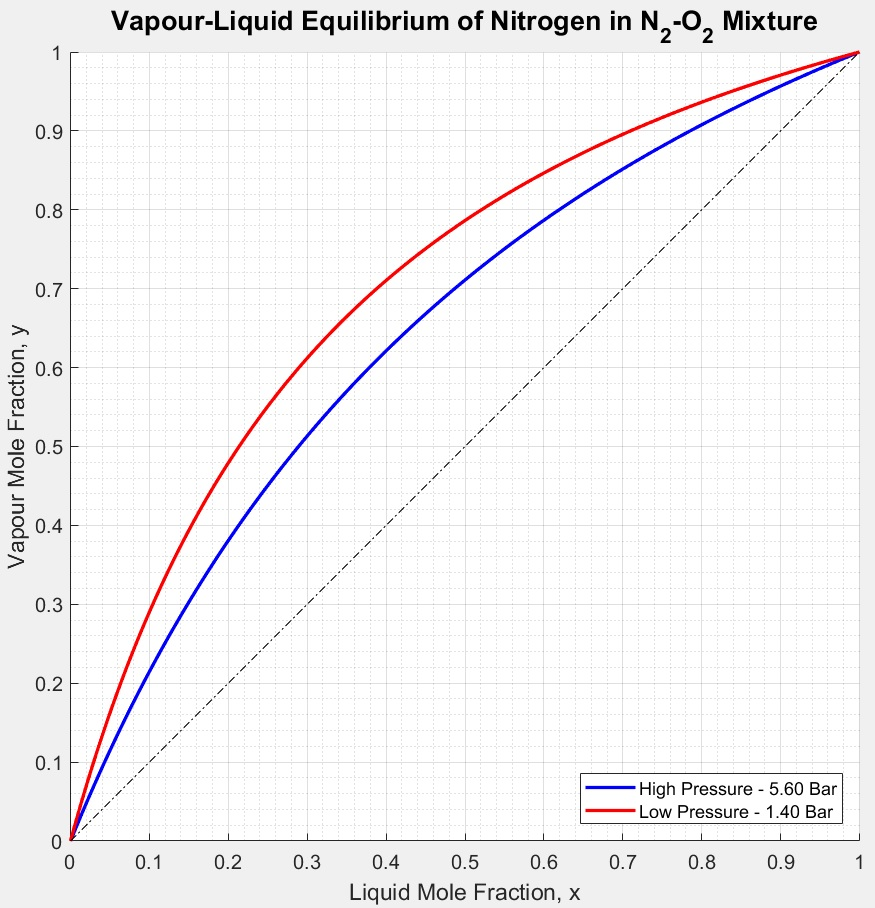
\includegraphics[scale=0.5]{VLEdata.jpg}
	        \caption{Vapour-Liquid Equilibrium of nitrogen in nitrogen-oxygen mixture}
	        \label{VLEdata}
        \end{figure}
        
        \noindent From the figure \ref{VLEdata}, we see that the VLE line at lower pressures moves away form the hypothetical $y=x$ dotted line, implying the nitrogen vapour is more enriched at lower pressures; this benefit, however, is offset by the lower boiling points at lower pressures. Hence a two-column design can allow a preliminary distillation in HPC (at 5.6 bar and 95.28 K) before a further purification in LPC (at 1.4 bar and 80.40 K). \\
        McCabe-Thiele Construction can be used to calculate the number of equilibrium stages required for separation in the two columns, by setting the distillate and bottom products' purities, with the following assumptions:
        \begin{enumerate}
            \item molar heat of vapourisation is the same for feed components at each independent equilibrium stage. Hence for each mole of vapour condensed, one mole of liquid is vapourised (i.e. equal molar overflow);
            \item vapour and liquid streams are assumed to be saturated at their respective boiling points with respect to their equilibrium position;
            \item negligible heat losses or mixing effects.
        \end{enumerate}
        By specifying the purity requirements and feed condition(s), operating lines and feed line(s) can be found by taking control volumes and considering mass balances around different sections of the column and feed inlets. Figure \ref{labelled_columns_diagram} shows the variables used for operating lines and feed lines functions.
        \begin{figure}[H]
            \centering
            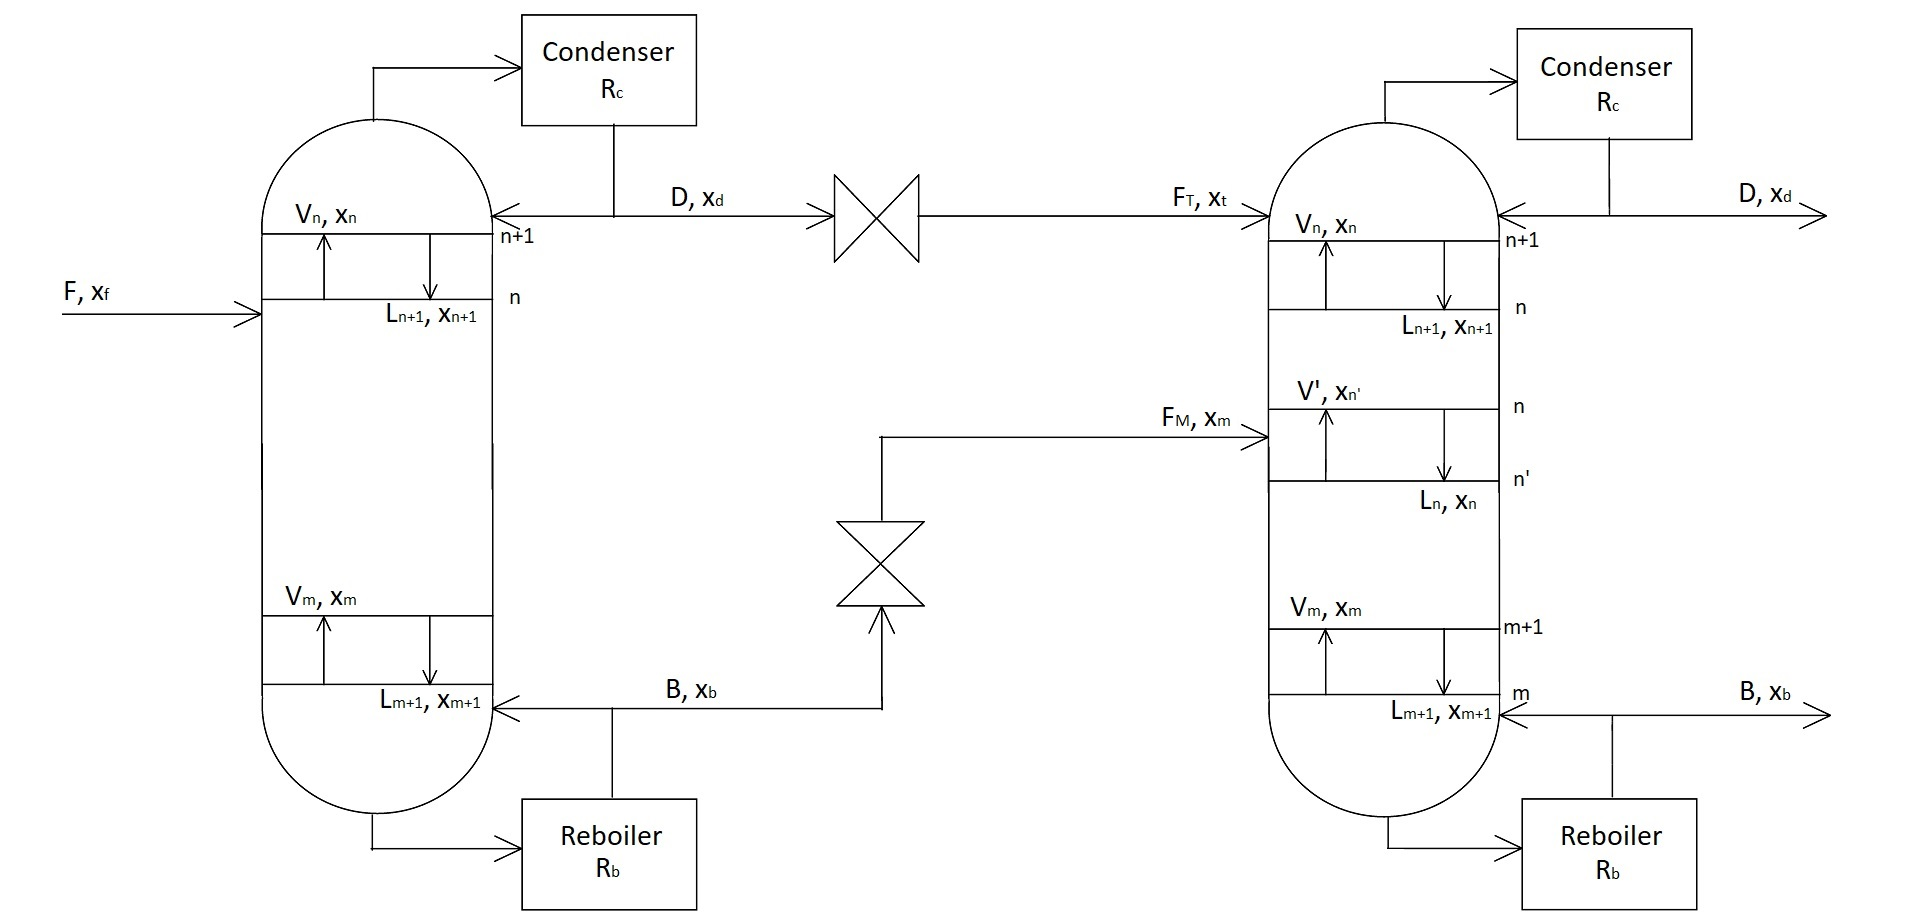
\includegraphics[scale=0.43]{labelled_columns_diagram.jpg}
            \caption{Diagrams of HPC and LPC with labels}
            \label{labelled_columns_diagram}
        \end{figure}
        \noindent Note that capital letters represent molar flow rates (with $L$ for Liquid, $V$ for Vapour, $D$ for Distillate, $B$ for Bottom, $F_T$ for Top Feed and $F_M$ for Middle Feed), whilst $x$ and $y$ represent liquid and vapour mole fractions respectively. \\
        With reference to figure \ref{labelled_columns_diagram}, top operating line (TOL, for rectifying section) and bottom operating line (BOL, for stripping section) are defined by equation \ref{eq:TOL} and \ref{eq:BOL}:
        \begin{equation}
            y_n = \left(\frac{L_{n+1}}{V_n}\right)x_{n+1} + \left(\frac{D}{V_n}\right)x_d
            \label{eq:TOL}
        \end{equation}
        \begin{equation}
            y_m = \left(\frac{L_{m+1}}{V_m}\right)x_{m+1} - \left(\frac{B}{V_m}\right)x_b
            \label{eq:BOL}
        \end{equation}
        where $n$ represents the stages at the top of the column and $m$ represents the stages at the bottom. \\
        Alternatively, TOL and BOL can be expressed in terms of condenser and reboiler reflux ratios, $R_c$ ($=\frac{L_{n+1}}{D}$) and $R_b$ ($=\frac{V_m}{B}$), giving equation \ref{eq:TOL2} and \ref{eq:BOL2}: \\
        \begin{equation}
            y_n = \left(\frac{R_c}{R_c+1}\right)x_{n+1} + \left(\frac{1}{R_c+1}\right)x_d
            \label{eq:TOL2}
        \end{equation}
        \begin{equation}
            y_m = \left(\frac{R_b+1}{R_b}\right)x_{m+1} - \left(\frac{1}{R_b}\right)x_b
            \label{eq:BOL2}
        \end{equation}
        Reflux ratios are chosen by multiplying the minimum reflux ratio the system requires by a factor $k$, hence $R=kR_{min}$, which is typically 1.2 to 1.5 times of minimum reflux ratio \citep{treybal2004}. With a higher reflux ratio, fewer trays are required for separation hence a shorter column and lower initial capital investment. The trade-off, however, is increased condenser and reboiler work hence higher running cost. A value for reflux ratio factor of 1.2 is chosen for the initial analysis. \\
        Feed line(s) (q-line) is defined by equation \ref{eq:qline}:
        \begin{equation}
            y_q = -\left(\frac{q}{1-q}\right)x_q + \left(\frac{1}{1-q}\right)x_f
            \label{eq:qline}
        \end{equation}
        where $q$ (=$\frac{h_d-h_f}{h_{vap}}$) is the heat needed to one mole of feed to saturated vapour condition divided by molar enthalpy of feed. Note that for fully saturated liquid, q = 1 hence q-line has infinite gradient and therefore will be a vertical line; for fully saturated vapour, q = 0 hence q-line has zero gradient and therefore will be a horizontal line.\\
        Applicable only to LPC, middle operating line (MOL, between the two feed inlets) is defined by equation \ref{eq:MOL}. \\
        \begin{equation}
            y' = \left(\frac{L'}{V'}\right)x' + \left(\frac{D}{V'}\right)x_d -  \left(\frac{F_T}{V'}\right)x_T
            \label{eq:MOL}
        \end{equation}
        
        \noindent Two useful information to have are minimum condenser reflux ratio and minimum theoretical number of equilibrium stages. Minimum condenser reflux ratio can be found by setting the operating lines to intersect the q-line on the vapour-liquid eqilibrium curve (i.e in a pinched condition at infinite equlibrium stages); whilst minimum theoretical number of equlibrium stages can be found by setting the column in total condenser reflux (i.e. at infinite reflux) such that operating lines align with $y=x$ line.\\
        For a real life application, the separation process may exhibit non-ideal behaviour due to uneven mixing or non-uniform vapour-liquid composition. \\
        The model can be improved by applying a Murphree Tray Efficiency of 70\% to ensure thorough separation at each equilibrium stage. Murphree Tray Efficiency can be directly apply to the steps of the McCabe-Thiele construction with equation \ref{eq:Emv}: \\
        \begin{equation}
            \begin{aligned}
                E_{mv} & = \frac{y_{out} - y_{in}}{y_{eq} - y_{in}} \\
                y_{out} & = E_{mv}\left(y_{eq}-y_{in}\right) + y_{in}
            \end{aligned}
            \label{eq:Emv}
        \end{equation}
        
        \noindent A MATLAB script was written to automatically follow the operating line functions and construct the McCabe-Thiele plots for both HPC and LPC, which can be used to calculate the number of stages required, reflux ratios used and feed locations. An initial simulation is ran to produce two McCabe-Thiele plots which are shown in figure \ref{fig:mccabe_v0}.\\
        \begin{figure}[H]
            \begin{subfigure}{0.49\textwidth}
                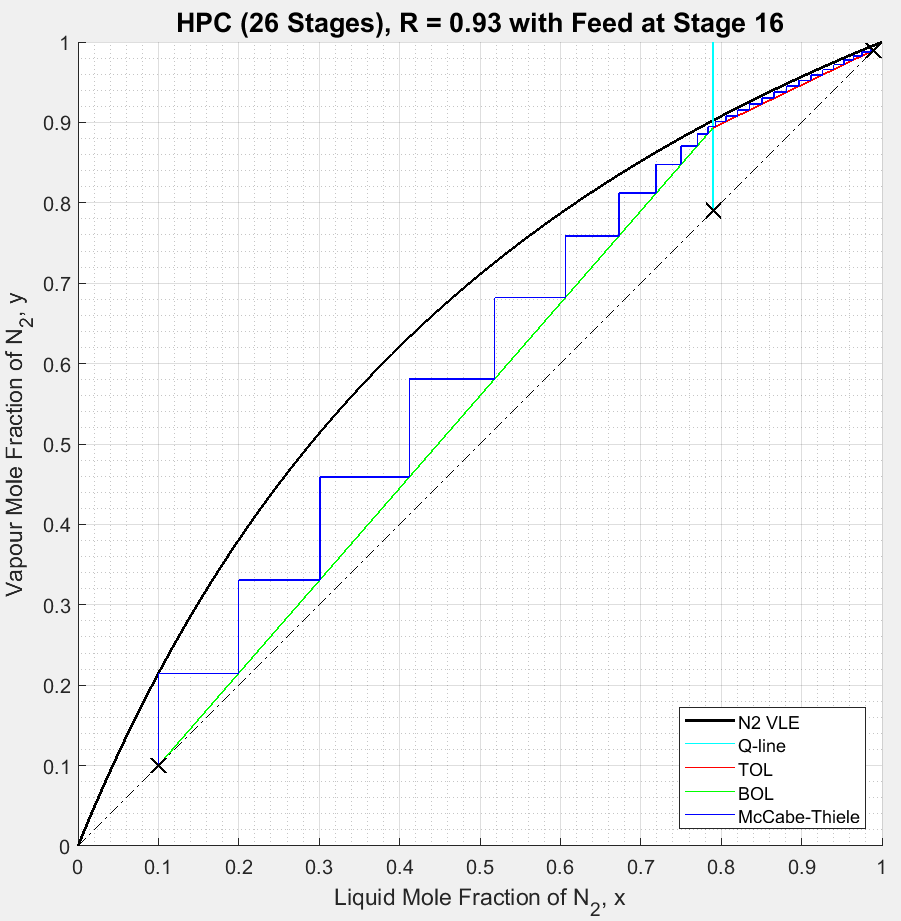
\includegraphics[width=\linewidth]{HPC_v0.jpeg}
                \caption{High Pressure Column}
                \label{fig:HPC_v0}
            \end{subfigure}
            \hspace*{\fill} % separation between the subfigures
            \begin{subfigure}{0.49\textwidth}
                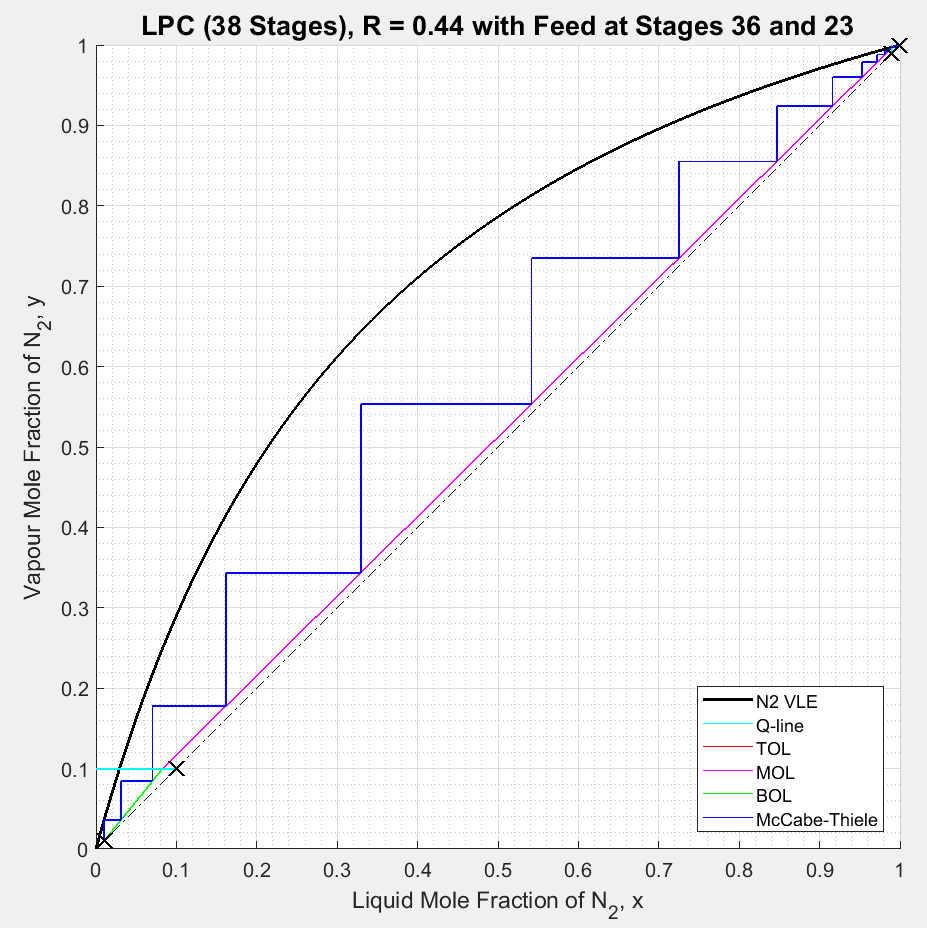
\includegraphics[width=\linewidth]{LPC_v0.jpeg}
                \caption{Low Pressure Column}
                \label{fig:LPC_v0}
            \end{subfigure}
            \caption{McCabe-Thiele Construction}                        \label{fig:mccabe_v0}
        \end{figure}
        \noindent Figure \ref{fig:HPC_v0} shows the McCabe-Thiele construction for the initial HPC design with the following parameters (on the basis of nitrogen purity):
        \begin{enumerate}
            \item Feed purity $x_f$ = 79\% (fully saturated liquid)
            \item Distillate purity $x_d$ = 99\% ($=x_t$ in LPC)
            \item Bottom purity $x_b$ = 10\% ($=x_m$ in LPC)
            \item Minimum condenser reflux ratio $R_{min}$ = 0.93 ($R = 1.2R_{min}$)
        \end{enumerate}
        Feed is assumed to be fully saturated liquid as the stream enters the column for separation, and two product streams are extracted from top and bottom of the column. In this configuration, mole flow rates $D$ = 0.0822 kmol/s and $B$ = 0.0238 kmol/s. \\
        As this is the first stage of distillation, distillate stream of HPC is used as the top feed for LPC and bottom stream of HPC is used as the middle feed for LPC, for a second stage of purification.\\
        \\
        Distillate and bottom streams are put through separate throttles to lower their pressures, transitioning from 5.6 bar to 1.4 bar, in between HPC and LPC. As distillate stream is assumed to be fully saturated liquid whilst bottom stream is assumed to be fully saturated vapour, isentropic expansion in the throttles induce saturated liquid-vapour states in both streams. The processes can be visualised by figure \ref{transition_T-S_diagram}. \\
        \begin{figure}[H]
            \centering
	        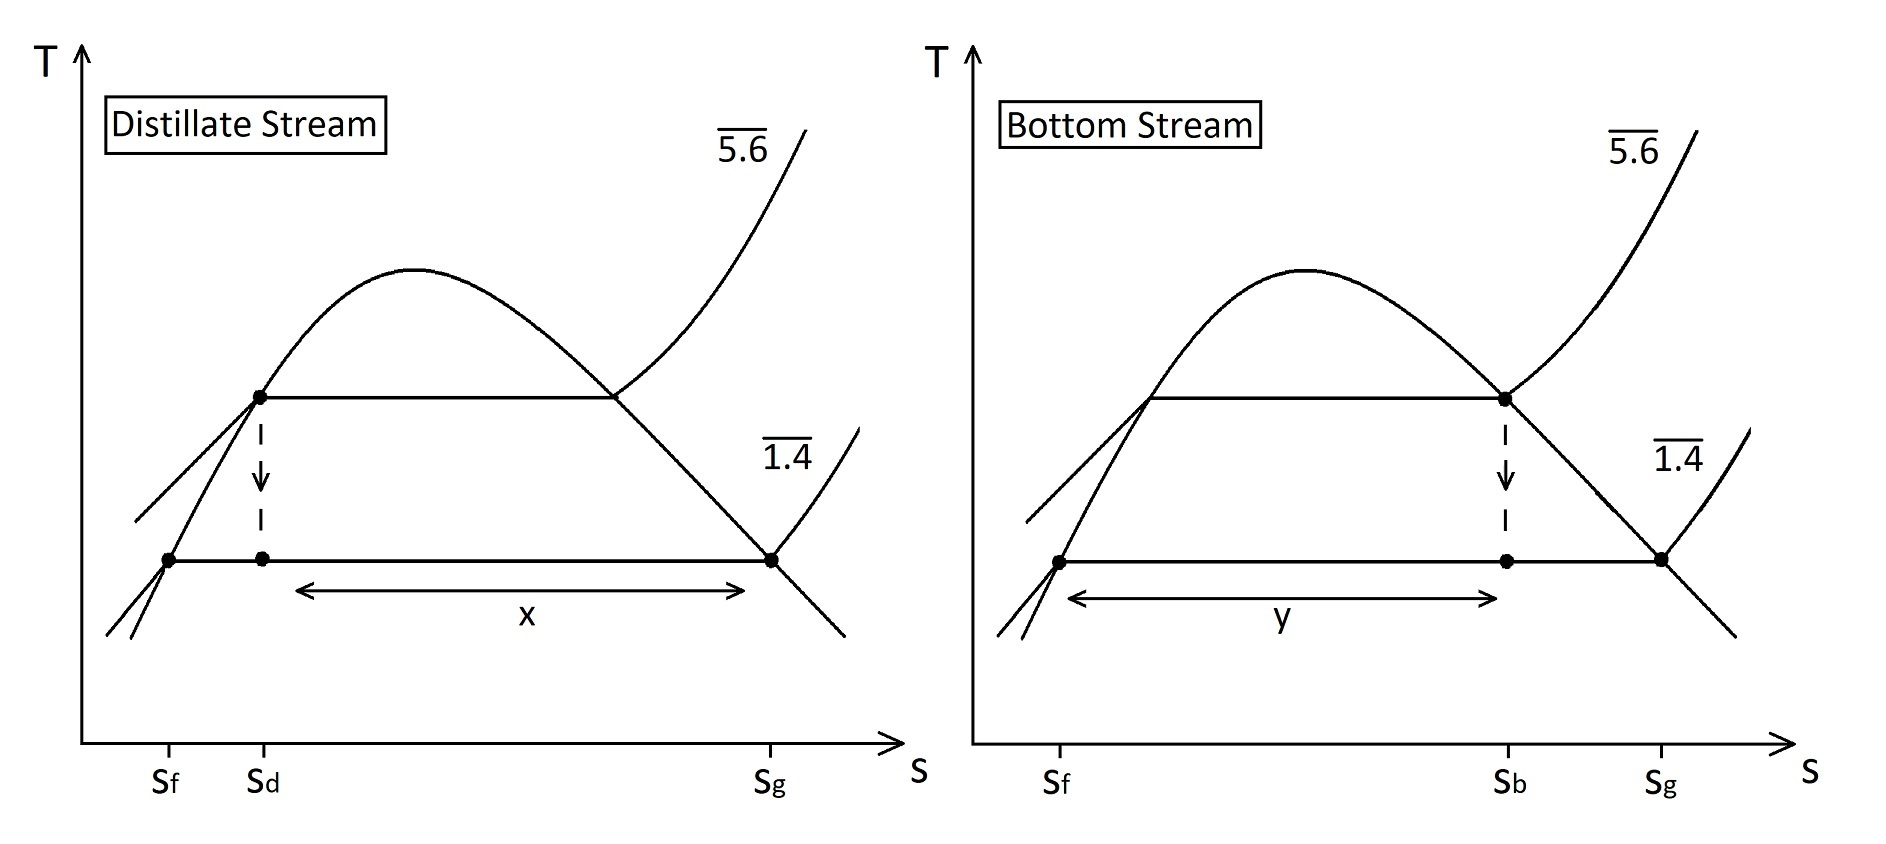
\includegraphics[width=1.00\linewidth]{transition_T-S_diagram.jpg}
	        \caption{Temperature-Entropy Diagram of the Transition in between HPC and LPC}
	        \label{transition_T-S_diagram}
        \end{figure} 
        \noindent Through the use of equations \ref{eq:transition_xy},
        \begin{equation}
            \begin{aligned}
                x = \frac{s_d-s_g}{s_f-s_g} \\
                y = \frac{s_b-s_f}{s_g-s_f}
            \end{aligned}
            \label{eq:transition_xy}
        \end{equation}
        and entropy data in table \ref{table:transition_entropy}, liquid fraction $x$ (correspond to distillate stream) and vapour fraction $y$ (bottom stream) can be found. \\
        \begin{table}[H]
        \centering
            \singlespacing
	        \caption{Entropy Data for Distillate and Bottom Stream}
	        \label{table:transition_entropy}
	
	        \begin{tabular}{|l|c|cc|c|}
	        \hline
	        Stream      	& $s_i$ (5.6 bar)   & $s_f$ (1.4 bar)   & $s_g$ (1.4 bar)   & $x$ or $y$     \\
	        \hline
	        Distillate		& 91.841			& 81.611            & 149.892           & 85\% \\
	        Bottom			& 159.956   	    & 95.892            & 167.748           & 89\% \\
	        \hline
	        \end{tabular}
        \end{table}
        \noindent This shows that neither of the streams are fully saturated, as distillate stream contains 85\% saturated liquid and bottom stream contains 89\% saturated vapour after throttling. This implies that the feed lines will no longer be perfectly vertical (fully saturated liquid) or horizontal (fully saturated vapour); but with only a 10\% difference, there is an observable difference but the impact on the separation process should be small. Hence for simplicity of analysis, both streams are assumed to be fully saturated when they enter LPC.\\
        \\
        Figure \ref{fig:LPC_v0} shows the McCabe-Thiele construction for the initial LPC design with the following parameters (on the basis of nitrogen purity):
        \begin{enumerate}
            \item Top feed purity $x_t$ = 99\% (fully saturated liquid)
            \item Middle feed purity $x_m$ = 10 \% (fully saturated vapour)
            \item Distillate purity $x_d$ = 99.99\%
            \item Bottom purity $x_b$ = 1\%
            \item Minimum condenser reflux ratio $R_{min}$ = 0.44 ($R = 1.2R_{min}$)
        \end{enumerate}
        Top feed is assumed to be fully saturated liquid and middle feed is assumed to be fully saturated vapour as the streams enter the column for purification. This allows two purified product streams to be extracted from top and bottom of the column. In this configuration, mole flow rates $D$ = 0.0836 kmol/s and $B$ = 0.0225 kmol/s. \\
        Although this design satisfies the product streams purity and supply requirements,  operating lines in LPC are near total reflux conditions despite only running at 1.2 times of minimum reflux ratio. This is due to the fact that HPC produces a much larger distillate stream than bottom stream, which contributed to the imbalance of vapour and liquid feed streams as inputs to LPC. \\
        \\
        The two major contributors to the cost of operation of the distillation columns are the number of equilibrium stages in the columns and the reflux ratios the columns are running at. The number of equilibrium stages directly relates to the dimensions of the column and insulation required, whilst the reflux ratios directly relate to the reboiler and condenser thermal loads and sizes. \\
        In order to reduce the column operational cost, further investigation into the design details of the column will be discussed in the next section.
		\subsubsubsection{Distillation Column Reboiler and Condenser}
		The two-column system uses two sets of reboiler and condenser units to regenerate liquid and vapour flows in the columns. As the liquid mixture flows down the column and gathers at the bottom, a portion of the flow is vapourised by the reboiler and forms the rising vapour stream. Similarly, the vapour stream rising to the top of the column is condensed by the condenser to replenish the liquid stream. This forms the cycle of stripping and rectifying in the column. \\
		
	    \noindent There is an integrated design between HPC condenser and LPC reboiler. Adopted from Linde Engineering cryogenic plant \citep{linde_cryo}, the design is redrawn in figure \ref{reboiler-condenser_diagram}. \\
		\begin{figure}[H]
		    \centering
		    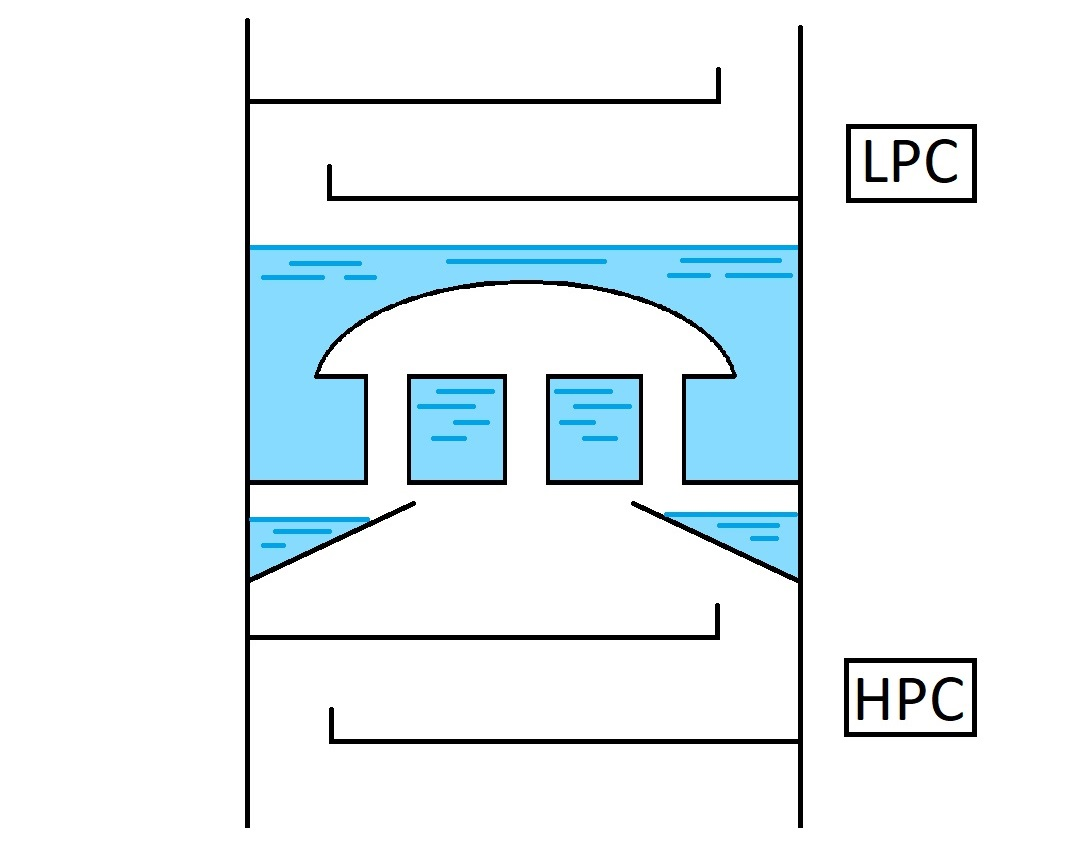
\includegraphics[scale=0.3]{reboiler-condenser_diagram.jpg}
		    \caption{Special Inter-Column Reboiler-Condenser Configuration}
		    \label{reboiler-condenser_diagram}
		\end{figure}
	    \noindent The boiling point of pure nitrogen at 5.6 bar is higher than the boiling point of pure oxygen at 1.4 bar, hence the refrigeration required to condense nitrogen at the top of HPC can be supplied by boiling the oxygen at the bottom of LPC. This replenishes both the liquid stream in HPC and vapour stream in LPC. With this configuration, no external thermal load is required, hence it maximises the thermal efficiency of the system. \\
\subsection{Analysis} \noindent
This section details the process to improve the system by optimising the two-column design and balancing heat of streams.
	\subsubsection{Distillation Column Optimisation} \noindent
	In the "Distillation Column" section, a preliminary set of parameters are introduced to allow initial analysis of the distillation. The set of parameters are as follows:
    \begin{enumerate}
        \item HPC distillate purity $x_d$ = 99\% ($=x_t$ in LPC)
        \item HPC bottom purity $x_b$ = 10\% ($=x_m$ in LPC)
        \item Reflux ratio factor $k$ = 1.2 (applies to both columns)
    \end{enumerate}
    As shown previously, the system running at this set of parameters is not very efficient. It can be improved by running simulations on different parameters and hence find an optimal set of operating conditions.
    \subsubsubsection{HPC Distillate Stream Purity}
    The first parameter to optimise is the HPC distillate stream purity $x_d$. The distillate stream of HPC is the first step for nitrogen purification. It is to be isentropically expanded in a throttle before entering the rectifying section of LPC, forming the main body of the liquid stream travelling down the column. \\
    Simulations are to be ran at HPC bottom purity $x_B$ of 10\% and reflux ratio factor $k$ of 1.2. The minimum distillate purity allowed by the VLE curve is 90\%, hence simulations are ran at 1\% interval in the range of 90\% to 99\% to test out the impact on the system. \\
    
    \noindent Figure \ref{fig:optimisation_1a} shows the change in number of stages required by the system, while figure \ref{fig:optimisation_1b} shows the change in reflux ratios required by system. \\
    \begin{figure}[ht]
        \centering
        \begin{subfigure}{0.49\textwidth}
            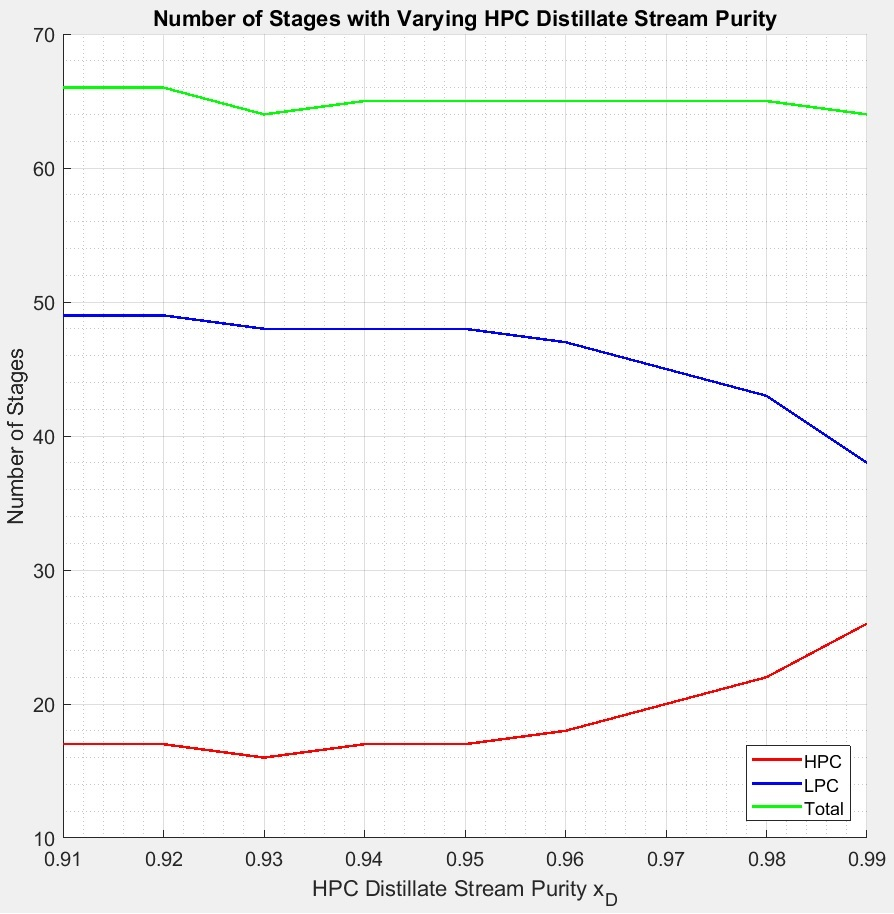
\includegraphics[width=\linewidth]{graph-stages_vs_HPCxD.jpg}
            \caption{Number of Stages} \label{fig:optimisation_1a}
        \end{subfigure}
        \hspace*{\fill} % separation between the subfigures
        \begin{subfigure}{0.49\textwidth}
            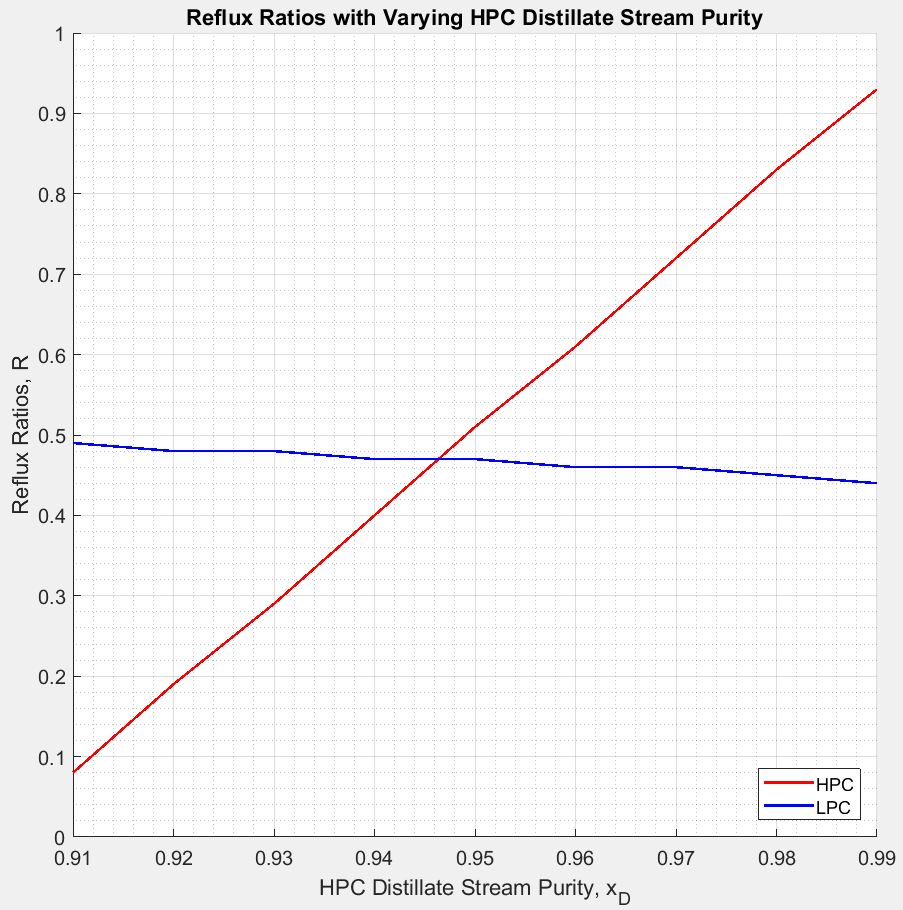
\includegraphics[width=\linewidth]{graph-reflux_vs_HPCxD.jpeg}
            \caption{Reflux Ratios} \label{fig:optimisation_1b}
        \end{subfigure}
        \caption{Optimising HPC Distillate Stream Purity} \label{fig:optimsation_1}
    \end{figure}
	\noindent From figure \ref{fig:optimisation_1a}, we see that as the purity $x_D$ increases, number of stages required by HPC (denoted by red line) increases whilst that of LPC (denoted by blue line) decreases. The total stages required (denoted by green line) stayed relatively constant, with the lowest number of stages required at purity of 93\% and 99\%. \\
	From figure \ref{fig:optimisation_1b}, we see that as the purity $x_D$ increases, reflux ratios required by HPC (red) increases rapidly whilst that of LPC (blue) decreases slightly. \\
	An extra set of data on the stream flow rates between the two columns is also generated, which showed insignificant changes and hence is not presented.\\
	Considering the effects on the number of stages and reflux ratios by running simulation on HPC distillate purity, I have chosen 93\% to be the optimal condition.
	\subsubsubsection{HPC Bottom Stream Purity}
    The second parameter to optimise is the HPC bottom stream purity $x_d$. The bottom stream of HPC is the first step for oxygen purification. It is to be isentropically expanded in a throttle before entering the stripping section of LPC, forming the main body vapour stream travelling up the column. \\
    Simulations are to be ran at HPC distillate purity $x_D$ of 93\% and reflux ratio factor $k$ of 1.2. The minimum bottom purity allowed by the VLE curve is 70\%, hence simulations are ran at 10\% interval in the range of 10\% to 70\% to test out the impact on the system. \\
    
    \noindent Figure \ref{fig:optimisation_2a} shows the change in number of stages required by the system, while figure \ref{fig:optimisation_2b} shows the change in stream flow rates in between the two columns. \\
    \begin{figure}[ht]
        \centering
        \begin{subfigure}{0.49\textwidth}
            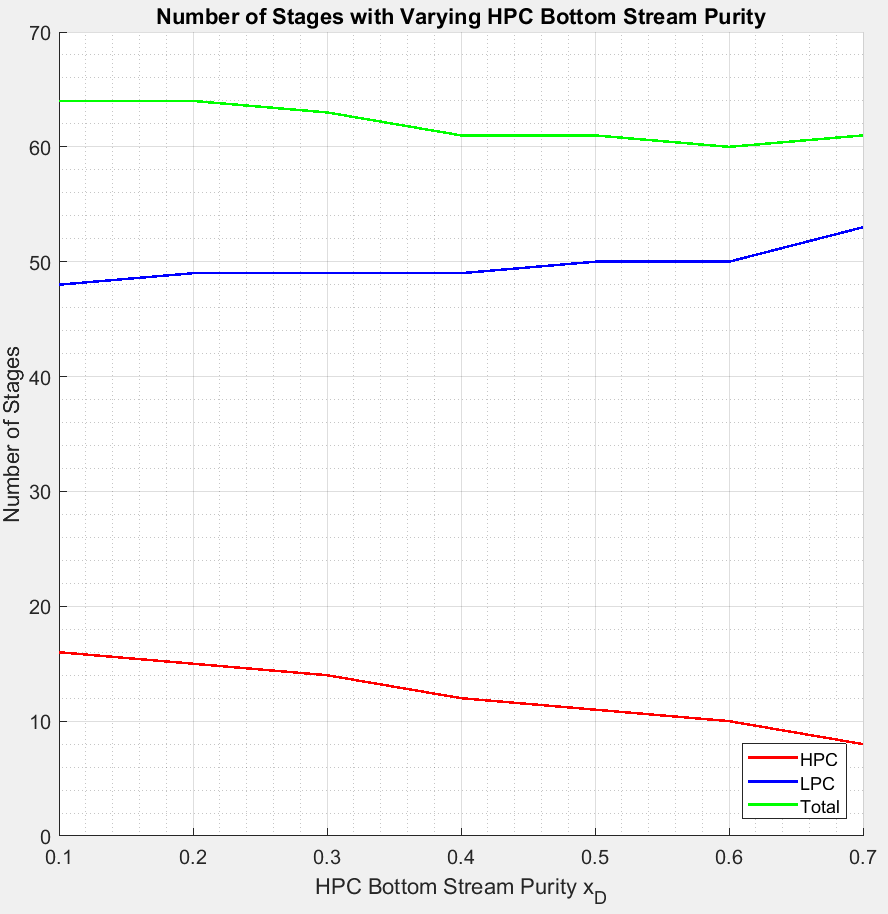
\includegraphics[width=\linewidth]{graph-stages_vs_HPCxB.jpeg}
            \caption{Number of Stages} \label{fig:optimisation_2a}
        \end{subfigure}
        \hspace*{\fill} % separation between the subfigures
        \begin{subfigure}{0.49\textwidth}
            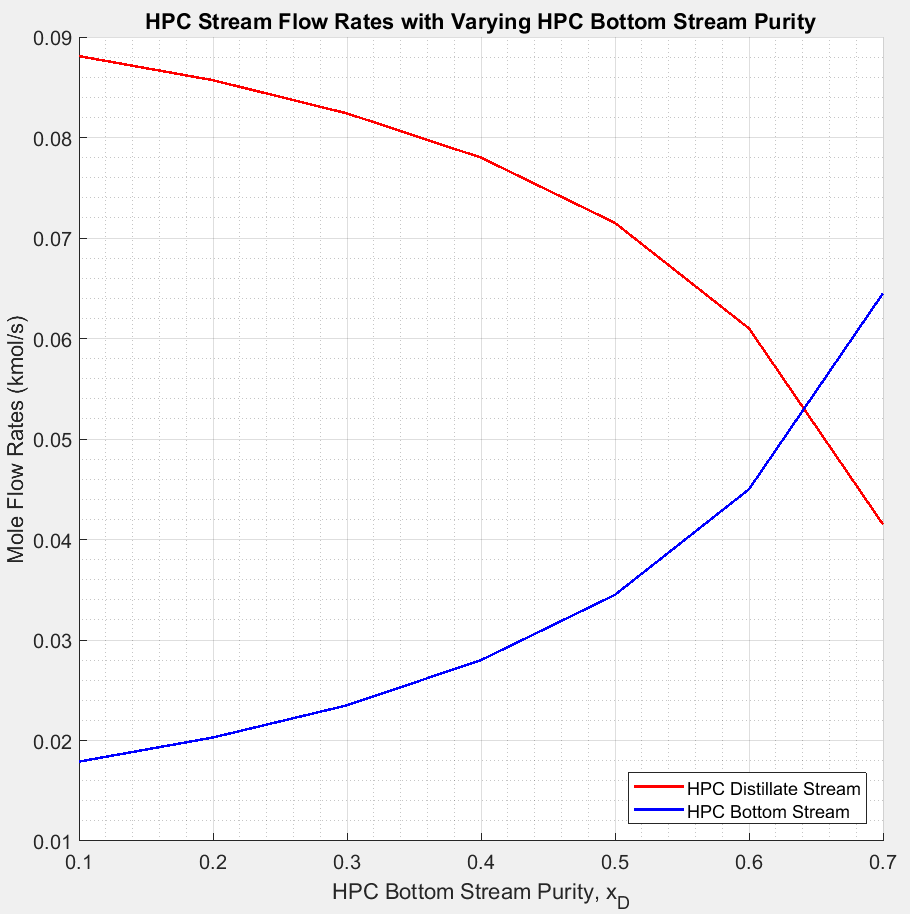
\includegraphics[width=\linewidth]{graph-flowrate_vs_HPCxB.jpeg}
            \caption{Stream Flow Rates} \label{fig:optimisation_2b}
        \end{subfigure}
        \caption{Optimising HPC Distillate Stream Purity} \label{fig:optimsation_2}
    \end{figure}
	From figure \ref{fig:optimisation_2a}, we see that as the purity $x_B$ increases, number of stages required by HPC (denoted by red line) decreases whilst that of LPC (denoted by blue line) increases. The total stages required (denoted by green line) stayed relatively constant, with the lowest number of stages required at purity of around 60\%. Further stimulation at 1\% interval between 60\% to 70\% showed that the lowest number of stages applies to purity conditions of 61\% to 65\%. \\
	From figure \ref{fig:optimisation_2b}, we see that as the purity $x_B$ increases, HPC distillate stream flow rate (denoted by red line) decreases whilst that of HPC bottom stream (denoted by blue line) increases. The two curves cross at 65\% purity, which implies equimolar flow out in top and bottom section of the column. This is a high-efficient condition as supply of vapour and liquid streams in LPC are matched, thus minimising reboiler and condenser duty.\\
	An extra set of data on the reflux ratios between the two columns is also generated, which showed no changes and hence is not presented.\\
	Considering the effects on the number of stages and HPC output stream flow rates by running simulation on HPC bottom purity, I have chosen 65\% to be the optimal condition.
    \subsubsubsection{Reflux Ratio Factor}
    The third parameter to optimise is the reflux ratio factors for both HPC and LPC. To simplify the analysis, the same reflux ratio factor is to be applied to both HPC and LPC. Simulations are to ran at HPC distillate purity $x_D$ of 93\% and HPC bottom purity $x_B$ of 65\%. From \cite{treybal2004}, optimum reflux ratios are often within the range of 1.2 to 1.5 times of minimum reflux ratio, but for cryogenic system this might not be the case (discussion with Prof. Nick Hankins on 13th Feb, 2018); hence simulations are ran at 0.1 interval in the range of 1.1 to 2.0 to test out the impact on the system.
    \begin{figure}[H]
        \centering
        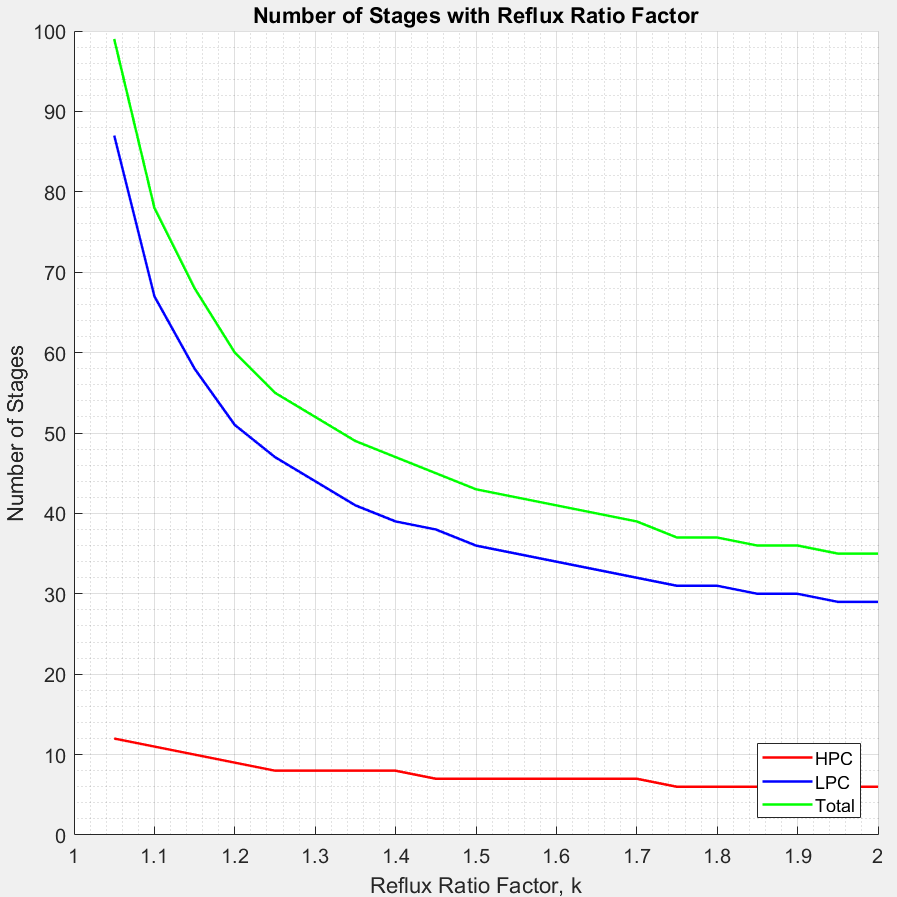
\includegraphics[width=0.45\linewidth]{graph-stages_vs_R.jpeg}
        \caption{Number of Stages}
        \label{fig:optimisation_3}
    \end{figure}
	\noindent From figure \ref{fig:optimisation_3}, we see that as the reflux ratio factor $k$ increases, number of stages required by HPC (denoted by red line) decreases slightly whilst that of LPC (denoted by blue line) decreases rapidly. The total stages required (denoted by green line), heavily influenced by LPC, also decreases rapidly and plateaued towards factor of 2.0. \\
	As number of stages relates to column dimensions and reflux ratio factor relates to reboiler and condenser loads, this information will be used in the "Cost Analysis" session later.
    \subsubsection{Design Dimensions} \noindent
		\subsubsubsection{Heat Exchanger}
		Plate-fin heat exchangers are used to transfer heat between cold and hot streams. As a simplification to the analysis, condensers and reboilers are also modelled as heat exchangers. The surface area can be found using equation \ref{eq:hex}.
		\begin{equation}
		    A_s = \frac{\Delta Q}{U\Delta T_m}
		    \label{eq:hex}
		\end{equation} 
		where $U\Delta T_m$ is taken to be 11250 Btu hr$^{-1}$ft$^{-2}$ (or 35.49 kWm$^{-2}$).
		
		\subsubsubsection{Distillation Column}
		Design dimensions of the distillation columns are controlled by the reflux ratios. With higher reflux ratios, wider columns are needed to accommodate larger vapour and liquid streams inside the column; but the columns will be shorter as fewer equilibrium stages are needed. These two dimensions, diameter and height, can directly affect both the capital cost and the operating cost of the system. A cost analysis study is required to find an optimum balance between the two. \\
		
		\noindent In both HPC and LPC, a 24-inch (or 0.61 m) tray spacing assumption is used. It is common practice to leave additional spaces of 5 ft (or 1.52 m) both at the top of the column as vapour-liquid disengaging space and bottom as liquid sump \citep{douglas1988}. Equation \ref{eq:column_height} relates the height of the column $H$ (in m) to the number of equilibrium stages required $N$:
		\begin{equation}
		    H = 0.61N + 3.04;
		    \label{eq:column_height}
		\end{equation}
		The column diameter is selected to ensure vapour velocity is within 60\% of flooding velocity. Making the assumption that liquid density is much larger than vapour density, i.e. $\rho_f >> \rho_g$, vapour velocity can be expressed as equation \ref{eq:vapour_velocity} \citep{douglas1988}:
		\begin{equation}
		    v = \frac{F}{\sqrt{\rho_g}}
		    \label{eq:vapour_velocity}
		\end{equation}
		where F is a constant that can be found by carrying out force balance of weight against drag on an arbitrary particle. $F = 1.51$ is assumed for 24-inch tray spacing with 60\% flooding \citep{perry2007}. \\
		
		\noindent Volumetric flow rate $Q$ can be expressed in vapour molar flow rate $V$ and in vapour velocity $v$ in equation \ref{eq:volumetric_flow}. Equating these two equations and substituting in equation \ref{eq:vapour_velocity}, column diameter can be found in equation \ref{eq:column_diameter}.
		\begin{equation}
		    Q = \frac{V \cdot MW_g}{\rho_g} = \left(\frac{1}{4}\pi D^2\right)v
		    \label{eq:volumetric_flow}
		\end{equation}
		\begin{equation}
		    D = \sqrt{\frac{4V\cdot MW_g}{\pi F \sqrt{\rho_g}}}
		    \label{eq:column_diameter}
		\end{equation}
		where vapour molar flow rate is linked to reflux ratio by $V = (R+1)D$, $MW_g$ is the molecular weight of gas and $\rho_g$ is the vapour density.
	\subsubsection{Cost Analysis} \noindent
	The costing of the system will be analysed using Guthrie correlations, which make use of a cost index commonly used in chemical process industries called Marshall and Swift Cost Index, or M\&S. Although the publishing of M\&S has been discontinued in scientific journal "Chemical Engineering" from 2012, Guthrie correlations can still provide a simple analysis on the total installed cost of each major component. \\
	Using past M\&S values from \cite{peters1991} and \cite{marshall_swift}, dating back to 1975, data showed a general linear trend that can be extrapolated to give a hypothetical M\&S value of around 1450 for the year 2018. This value will be used in the cost analysis in this section. \\
	
    \noindent Total installed cost of reboilers and condensers are modelled using equation \ref{eq:cost_hex}, assuming they act as independent heat exchangers to simplify analysis \citep{douglas1988}.
    \begin{equation}
	    C_{hex} = \left(\frac{M\&S}{280}\right)\left(101.3\right)\left(A_s^{0.65}\right)\cdot (2.29 + F_c)
	    \label{eq:cost_hex}
	\end{equation}
	where $A_s$ is the heat exchanger surface area and $F_c = 5.06$ is the overall correction factor that relates to design type (kettle reboiler), design pressure (sub-10-bar operation) and design material (stainless steel). Note that area in the equation is expressed in ft$^2$, hence a conversion factor is applied (ft$^2$ = 0.0929 m$^2$). \\
	
	\noindent Total installed cost of distillation column is separated into two costs, cost for the pressure vessels and cost for the internal components (e.g. trays), using equation \ref{eq:cost_distill_vessel} and \ref{eq:cost_distill_internal} respectively \citep{douglas1988}.
	\begin{equation}
	    C_{col,ves} = \left(\frac{M\&S}{280}\right)\left(101.9\right)\left(D^{1.066}\right)\left(H^{0.802}\right)\cdot (2.18 + F_c)
	    \label{eq:cost_distill_vessel}
	\end{equation}
	where $D$ is the distillation column diameter , $H$ is the distillation column height and $F_c = 2.36$ is the correction factor that relates to design material (stainless steel) and design pressure (sub-7-bar operation). Note that dimensions in the equation are expressed in ft and ft$^2$, hence a conversion factor is applied (1 ft = 0.3048 m).\\
	\begin{equation}
	    C_{col,int} = \left(\frac{M\&S}{280}\right)\left(4.7\right)\left(D^{1.55}\right)\left(H\right)\cdot F_c
	    \label{eq:cost_distill_internal}
	\end{equation}
	where $F_c = 4.50$ is the correction factor that relates to tray spacing (24-inch), tray type (bubble-cap trays) and tray material (stainless steel). \\
    
    \noindent Using cost equations \ref{eq:cost_hex}-\ref{eq:cost_distill_internal}, a graph of fixed and operating costs of running the two-column distillation system against reflux ratio factor $k$ is plotted, shown in figure \ref{fig:column_cost_vs_reflux}.
    With increasing reflux ratio factor, operating cost (i.e. condenser and reboiler duties) rises steadily whilst fixed cost (i.e. cost of distillation columns) decreases sharply at low factor values. The total cost of operation is the summation of both fixed and operating cost. A black cross on the graph indicates the minimum total cost of USD 676,000 at reflux ratio factor of 1.75, which is the optimum point of operation. \\
    \begin{figure}[H]
        \centering
        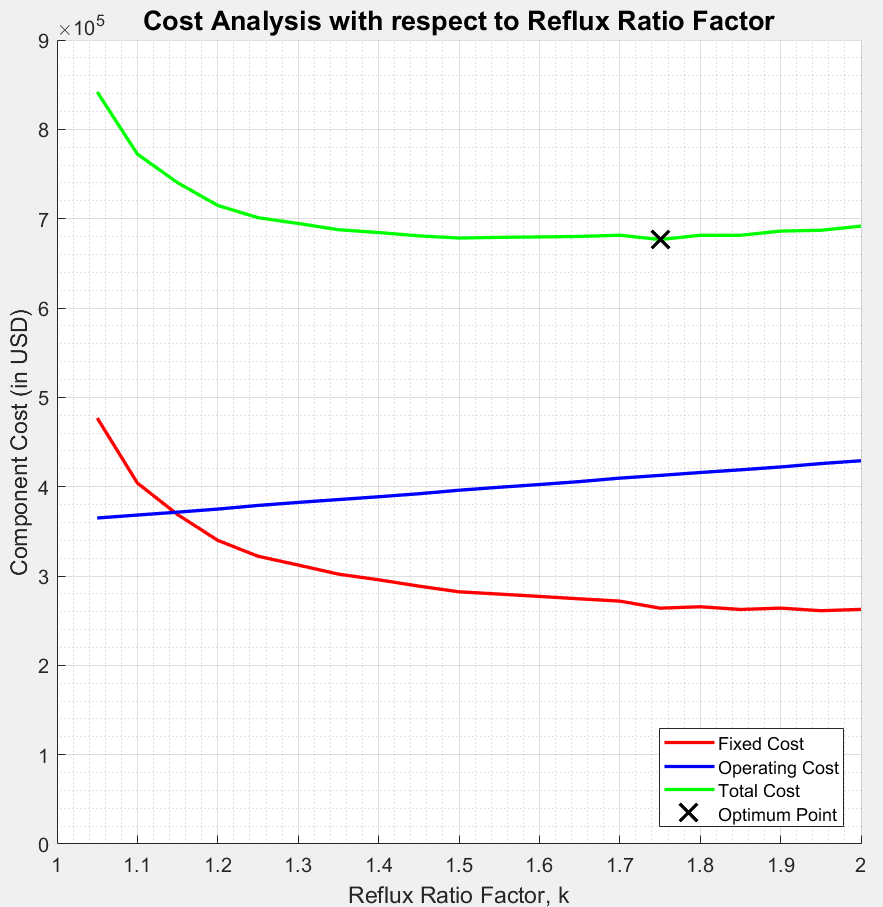
\includegraphics[scale=0.45]{column_cost_vs_reflux.jpeg}
        \caption{Distillation Column Cost with respect to varying Reflux Ratio Factor}
        \label{fig:column_cost_vs_reflux}
    \end{figure}
    \noindent With a reflux ratio factor of 1.75, new McCabe-Thiele plots can be generated for the two distillation columns, which are shown in figure \ref{fig:mccabe_v1}.
    \begin{figure}[H]
        \begin{subfigure}{0.49\textwidth}
            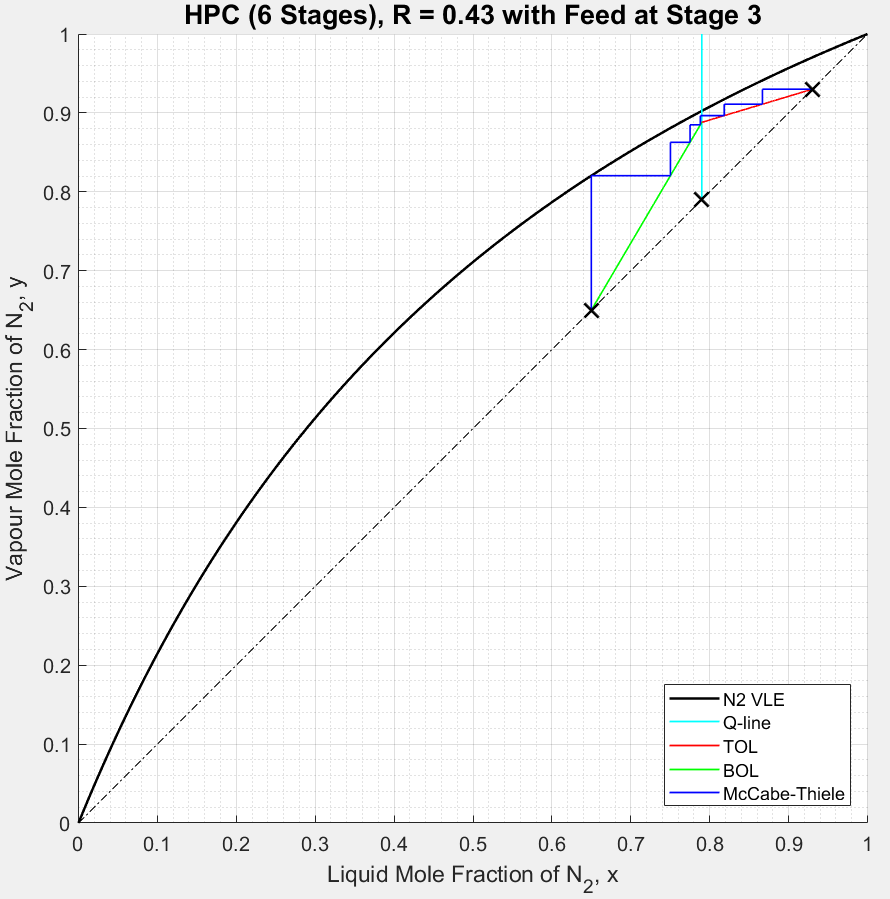
\includegraphics[width=\linewidth]{HPC_v1.jpeg}
            \caption{High Pressure Column}
            \label{fig:HPC_v1}
        \end{subfigure}
        \hspace*{\fill} % separation between the subfigures
        \begin{subfigure}{0.49\textwidth}
            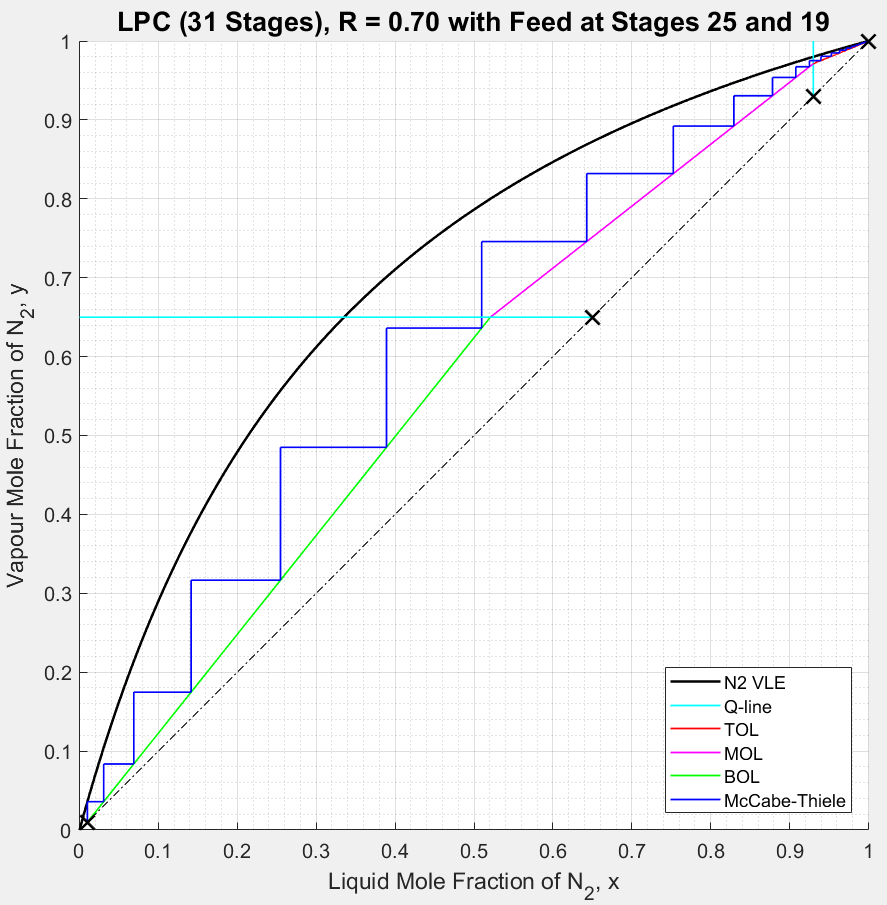
\includegraphics[width=\linewidth]{LPC_v1.jpeg}
            \caption{Low Pressure Column}
            \label{fig:LPC_v1}
        \end{subfigure}
        \caption{McCabe-Thiele Construction}                        \label{fig:mccabe_v1}
    \end{figure}
	\noindent Total installed cost of compressors can be found by \ref{eq:cost_compressor} \citep{douglas1988}. 
	\begin{equation}
	    C_{comp} = \left(\frac{M\&S}{280}\right)\left(517.5\right)\left(P^{0.82}\right)\cdot \left(2.11 + F_c\right)
	    \label{eq:cost_compressor}
	\end{equation}
	where $D$ is the distillation column diameter , $H$ is the distillation column height and $F_c = 1.00$ is the correction factor that relates to compressor design type (centrifugal compressor). Note that power in the equation is expressed in bhp, hence a conversion factor is applied (1 bhp = 0.7457 kW).
	\subsubsection{Heat Balance} \noindent \noindent
    For a cryogenic distillation system to be efficient, heat duties are to be kept internal within the distillation columns. Heat can be balanced and redistributed to warm up a cold stream (in a reboiler) or cool down a hot stream (in a condenser). \\ 
    The section "Liquefaction Unit" briefly discussed the use of LPC cold product streams to extract heat from inlet air stream, and summarised with a leftover of 728 kW of heat yet to be extract. The issue will be addressed in this section.
    \subsubsubsection{Reboiler and Condenser}
        Each distillation column has its own set of reboiler and condensers. For simplicity of analysis, they are modelled as heat exchangers such that their duty can be expressed as equation \ref{eq:heat_reboiler} and \ref{eq:heat_condenser} respectively, in terms of heat required for vaporise liquid at the top and bottom of the columns.
        \begin{subequations}
            \begin{equation}
                Q_{b} = V_m \cdot \tilde{h}_{fg} = BR_b \cdot \tilde{h}_{fg}
                \label{eq:heat_reboiler}
            \end{equation}
            \begin{equation}
                Q_{c} = V_n \cdot \tilde{h}_{fg} = D(R_c+1) \cdot \tilde{h}_{fg}
                \label{eq:heat_condenser}
            \end{equation}
		\end{subequations}
		where $\tilde{h}_{fg}$ is the vaporisation heat of mixture, as generalised by equation $\tilde{h}_{fg} = xh_{fg,N_2} + (1-x)h_{fg,O_2}$. \\
		
		\noindent Running both columns at reflux ratio factor of 1.75, duty and outlet stream temperatures are tabulated in table \ref{table:duty} \citep{nist}.
		\begin{table}[H]
        \centering
            \singlespacing
	        \caption{HPC and LPC Heat Duty in kW [Temperature in K]}
	        \label{table:duty}
	
	        \begin{tabular}{|l|cc|}
	        \hline
    	                    & HPC	            & LPC \\    \hline
	        Condenser		& 368.75 [96.51]	& 678.81 [80.21] \\
	        Reboiler  		& -447.77 [100.7]	& -595.65 [93.40] \\    \hline
	        \end{tabular}
	        \vspace{1ex}
	        
	        \raggedright Note that positive heat duties represent heat extraction by the unit (i.e. stream is cooled down) whilst negative heat duties represent heat addition (i.e. stream is heated up).
        \end{table}
        \noindent As previously discussed in section "Distillation Column Reboiler and Condenser", heat extraction required in HPC condenser can be supplied by LPC reboiler, whilst the heat addition in reboilers can be supplied by heat exchange with inlet air stream.
	    \subsubsubsection{Outlet Streams}
	    Outlet streams are considered cold when compared to inlet air stream, with LPC distillate stream at 80.21K and LPC bottom stream at 93.40K. \\
	    Amount of heat that can be extracted using the two streams can be expressed in equation \ref{eq:heat_outlet}.
	    \begin{equation}
	        \Delta Q = \dot{m}c_p \left(T_{out} - T_{in}\right)
	        \label{eq:heat_outlet}
	    \end{equation}
        where specific heat capacity $c_p$ = 57.62 Jmol$^{-1}$K$^{-1}$ for distillate stream (value for pure nitrogen at 1.4 bar) and $c_p$ = 54.69 Jmol$^{-1}$K$^{-1}$ for bottom stream (oxygen at 1.4 bar) \citep{nist}. $T_{out}$ is taken to be 288K as the streams exit the plant. \\
        Using equation \ref{eq:heat_outlet}, distillate stream can extract 1001 kW of heat whilst bottom stream can extract 239 kW of heat, which is more than the 728 kW of heat extraction required.
	\subsubsection{Control} \noindent
    	There are several important parameters to control in a cryogenic plant, e.g. input and output flow rates and product streams' purity. As the cryogenic distillation system is designed for a specific flow rate to produce high-purity nitrogen for the Haber-Bosch plant downstream, the main focus of the control session will be on the distillate flow rate of the system.\\
    	A conventional reference tracking control loop is shown in figure \ref{fig:control_loop}.
    	\begin{figure}[H]
    	    \centering
    	    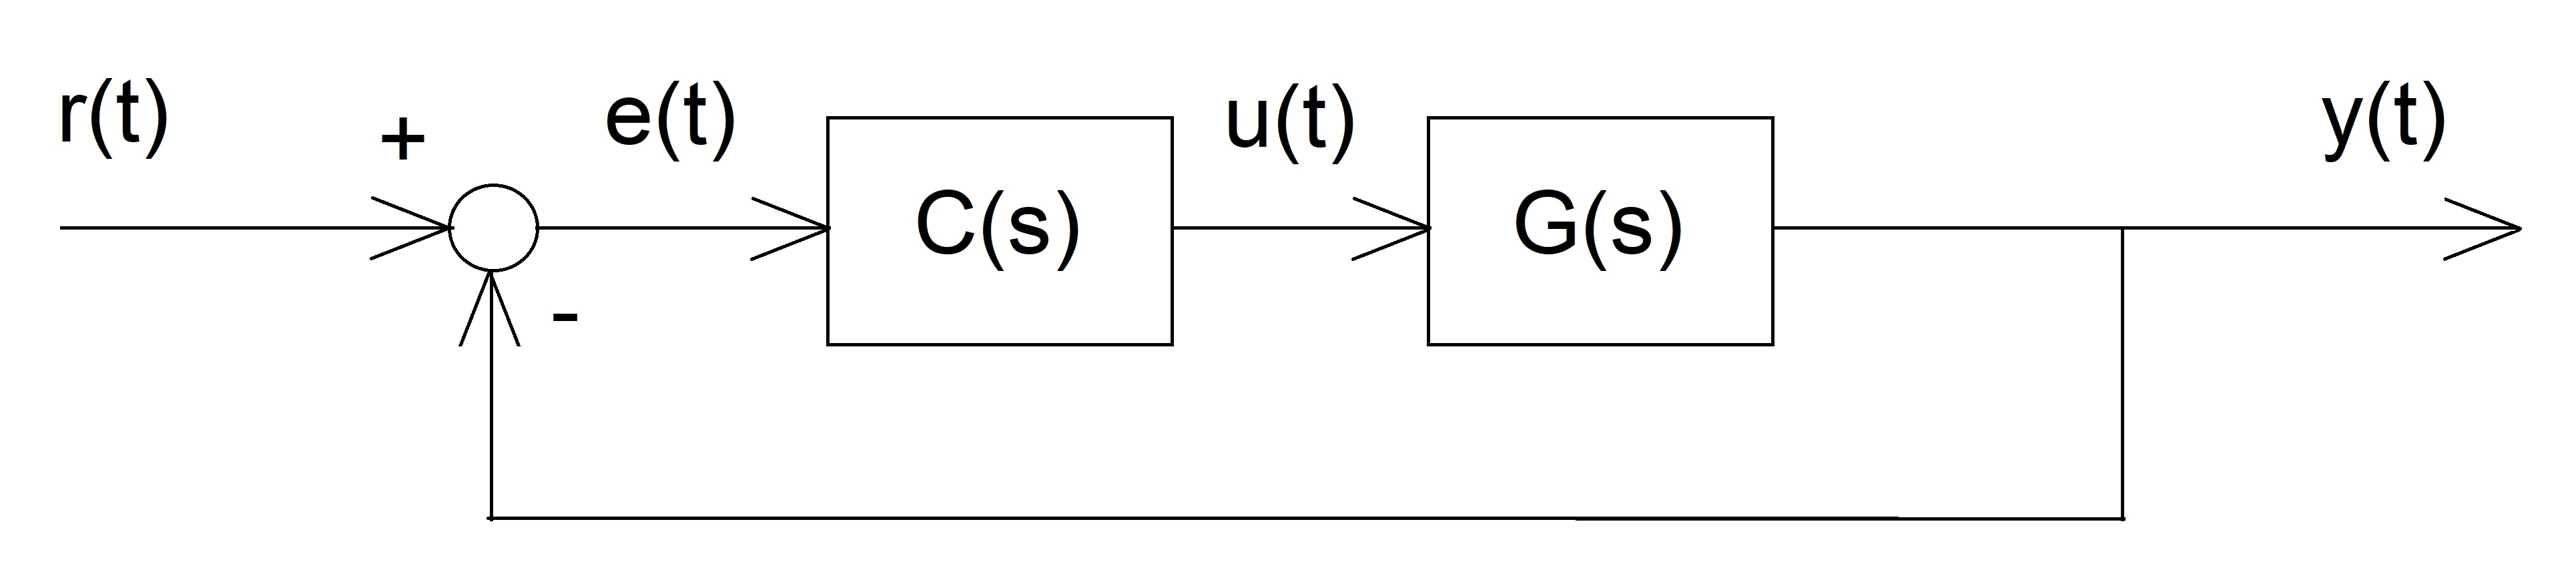
\includegraphics[width=0.7\textwidth]{control_loop.jpg}
    	    \caption{Simple Control Loop for Reference Tracking}
    	    \label{fig:control_loop}
    	\end{figure}
    	\noindent System can be modelled using a second-order transfer function, generalised in equation \ref{eq:transfer} \citep{control_transfer_function}.
    	\begin{equation}
    	    G(s) = \frac{Ke^{-Ds}}{(1+\tau _1s)(1+\tau _2s)}
    	    \label{eq:transfer}
    	\end{equation}
    	where $K$ is the steady-state gain, $D$ is the dead-time of the system and time coefficients are the lag-time. \\
    	Using time coefficients from a similar plant, the values are $\tau _1 = 250$ mins and $\tau _2 = 15$ mins respectively \citep{control_time_coefficient}. And for simplicity of analysis, it is assumed that $K = 1$ and $D = 0$.\\
    	For controller $C(s)$, a Proportional-Integral-Derivative (PID) controller will be used, generalised in equation \ref{eq:controller}.
    	\begin{equation}
    	    C(s) = P+I\frac{1}{s}+D\frac{N}{1+N\frac{1}{s}}
    	    \label{eq:controller}
    	\end{equation}
    	A step input is used and the control loop is modelled on Simulink, where $P$, $I$, $D$ and $N$ values are found using the Simulink tuner. These values, along with the controller performance, are tabulated in table \ref{table:control}.
        \begin{table}[H]
            \singlespacing
            \caption{PID Controller}
            \label{table:control}
            \begin{subtable}{.49\linewidth}
              \centering
                \caption{Parameters}
                \begin{tabular}{|p{0.8cm}|p{1.5cm}|}
                \hline
                P & 1.4197 \\
                I & 0.0100 \\
                D & -1.7761 \\
                N & 0.7993  \\
                \hline
                \end{tabular}
            \end{subtable}%
            \begin{subtable}{.49\linewidth}
              \centering
                \caption{Performance}
                \begin{tabular}{|p{2.5cm}|p{1.6cm}|}
                \hline
                Rise Time & 209 min \\
                Peak Time & 471 min \\
                Settling Time & 782 min \\
                Overshoot & 7.19\%  \\
                \hline
                \end{tabular}
            \end{subtable} 
        \end{table}
    	\noindent Figure \ref{fig:control_graph} shows the transient performance of the control loop, showing highly unresponsive behaviour to step changes. Settling time of around 12 hours implies that the column should not be subjected to changes lightly.  
    	\begin{figure}[H]
    	    \centering
    	    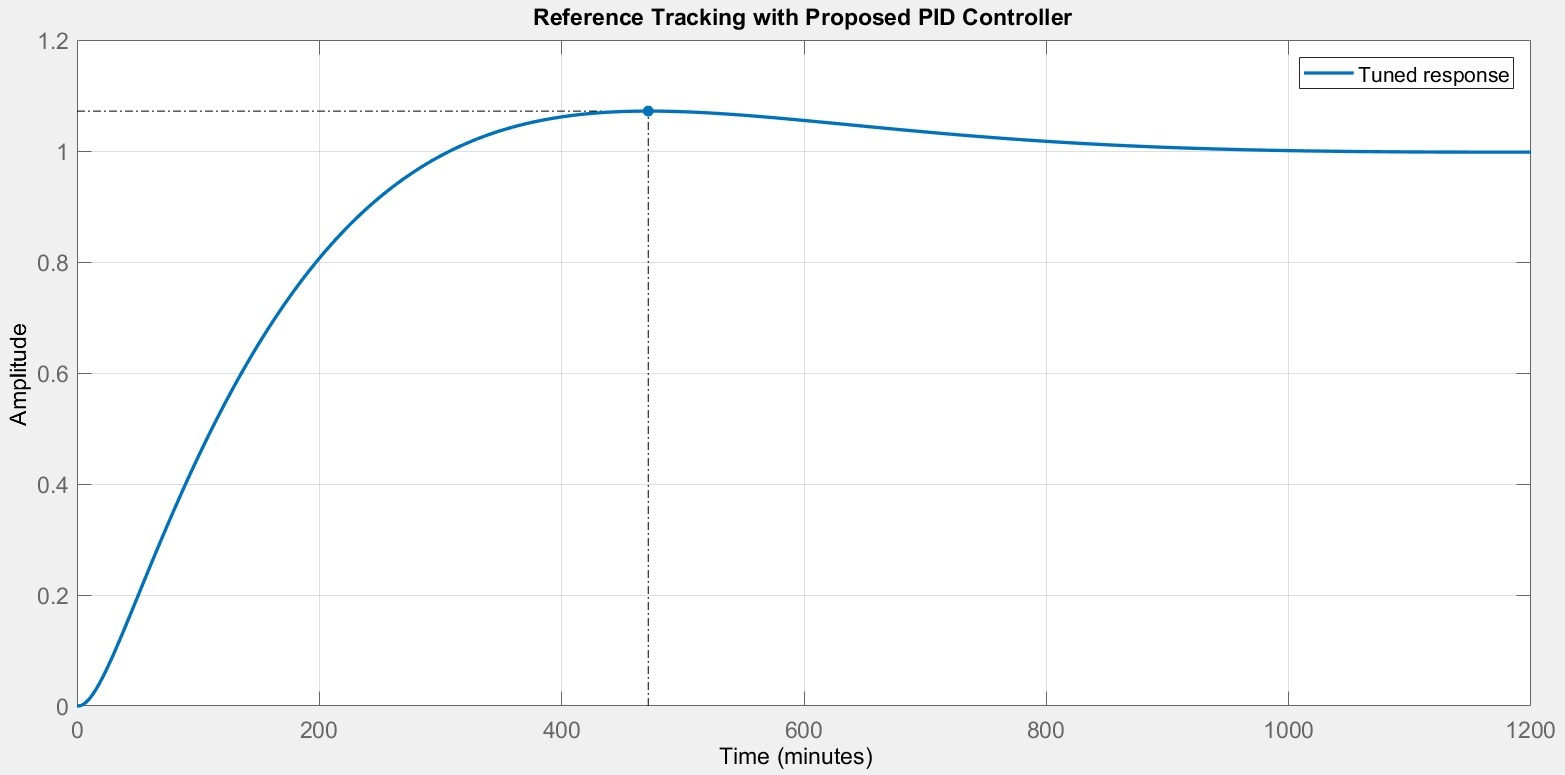
\includegraphics[width=0.75\linewidth]{graph-control.jpeg}
    	    \caption{Reference Tracking with Proposed PID Controller}
    	    \label{fig:control_graph}
    	\end{figure}
\subsection{Costing} \noindent
The main cost of running a cryogenic plant comes from the capital cost of compressors, capital cost of other components and operating cost of production are relatively low in comparison. \\
Most cryogenic distillation plants are designed to be self-sufficient by using hot and cold streams effectively, the plant is design to be independent from the grid, hence operating costs are essentially negligible.\\
A rough estimate on the costings of different plant components are summarised in table \ref{table:cost}.
\begin{table}[H]
    \singlespacing
    \centering
    \caption{Costing Estimate of Cryogenic Plant Components}
    \label{table:cost}
    \begin{tabular}{|l|r|}
        \hline
        Component                               & Cost (in USD)    \\     \hline
        Mechanical Air Filter \citep{matches}   & \$44,000         \\
        Molecular Sieve \citep{couper2012}      & \$92,000         \\
        Compressors \citep{matches}             & \$8,431,000      \\
        Heat Exchangers \citep{douglas1988}     & \$102,000        \\
        Separator \citep{matches}               & \$50,000         \\
        High Pressure Column \citep{douglas1988} & \$68,000         \\
        Low Pressure Column \citep{douglas1988}  & \$197,000        \\
        Condensers \citep{douglas1988}           & \$206,000        \\
        Reboilers \citep{douglas1988}            & \$207,000        \\     \hline
        Total                 & \$9,397,000     \\     \hline
    \end{tabular}
\end{table}

\subsection{Safety and Risk} \noindent
There are a few associated hazards when a cryogenic distillation plant is in operation, namely direct exposure to cryogenic material, oxygen-enriched air, asphyxiation in confined spaces and explosion due to rapid expansion of liquid. \\
To ensure the safety of workers and general public, a HAZOP study, tabulated in table \ref{table:HAZOP}, is conducted to identify sources of hazards and methods are devise to reduce the risks.
\subsection{Conclusion \& Further Work}
\noindent A double-column design is adopted to perform air separation and produce two high-purity product streams continuously. The cryogenic distillation plant is expected to produce 202.8 tpd of nitrogen at 99.99\% purity to be used to synthesize ammonia in Haber-Bosch plant downstream, and 62.7 tpd of oxygen at 99\% purity to be used in ammonia gas turbine. \\
For the plant to be implemented in reality, more in-depth analysis is required in several areas: column vessel and insulation materials, different operating conditions of columns, alternative liquefaction system and heat balance of streams. Regardless, this section on cryogenic distillation of air was overall successful.
\begin{landscape}
\begin{table}[p]
    \singlespacing
    \centering
    \caption{HAZOP Study of the Cryogenic Plant}
    \label{table:HAZOP}
    \begin{adjustbox}{width=\linewidth}
    \setlength{\extrarowheight}{8pt}
    \begin{tabular}{|l|l|l|l|l|}
    \hline
    Guideword & Deviation & Possible Causes & Consequences & Action Required \\ \hline
    NO & No feed & \begin{tabular}[c]{@{}l@{}}- Filter malfunction\\ - Obstruction in pipes or valves\\ - Compressor malfunction\end{tabular} & - Halted production & \begin{tabular}[c]{@{}l@{}}- Regular maintenance of pipes and valves\\ - Regular cleaning or replacement of filter\\ - Regular maintenance of compressor\end{tabular} \\ \hline
    LESS & Smaller feed stream & \begin{tabular}[c]{@{}l@{}}- Blocked filter\\ - Obstruction in pipes or valves\\ - Compressor malfunction\end{tabular} & - Smaller product streams & \begin{tabular}[c]{@{}l@{}}- Regular maintenance of pipes and valves\\ - Regular cleaning or replacement of filter\\ - Regular maintenance of compressor\end{tabular} \\ \hline
    LESS & Lower temperature in columns & \begin{tabular}[c]{@{}l@{}}- Heat-exchanger malfunction\\ - Reboiler malfunction\end{tabular} & \begin{tabular}[c]{@{}l@{}}- Flooding in trays and liquid sump\\ - Impure products\end{tabular} & \begin{tabular}[c]{@{}l@{}}- Regular maintenance of heat-exchanger and reboilers\\ - Regulate temperature with sensors\end{tabular} \\ \hline
    LESS & Lower pressure in columns & \begin{tabular}[c]{@{}l@{}}- Compressor malfunction\\ - Leakage in system\end{tabular} & \begin{tabular}[c]{@{}l@{}}- Impure products\\ - Escape of cryogenic materials\\ - Creation of oxygen-enriched/deficient atmosphere\end{tabular} & \begin{tabular}[c]{@{}l@{}}- Regular maintenance of compressors and leakage testing\\ - Regulate pressure with sensors\\ - Ensure good ventilation in confined spaces\end{tabular} \\ \hline
    MORE & Larger feed stream & \begin{tabular}[c]{@{}l@{}}- Damaged filter\\ - Compressor malfunction\end{tabular} & \begin{tabular}[c]{@{}l@{}}- Build up of material in system\\ - Impure products\end{tabular} & \begin{tabular}[c]{@{}l@{}}- Regular maintenance of compressor and replacement of filter\\ - Regulate flow with sensors\\ - Use of pressure-relief valves\end{tabular} \\ \hline
    MORE & Higher temperature in columns & \begin{tabular}[c]{@{}l@{}}- Intercooler malfunction\\ - Condenser malfunction\\ - Damaged column insulation\end{tabular} & \begin{tabular}[c]{@{}l@{}}- Expansion of liquid in columns\\ - Impure products\\ - Increased load on condensers\end{tabular} & \begin{tabular}[c]{@{}l@{}}- Regular maintenance of heat-exchanger and condensers\\ - Regulate temperature with sensors\end{tabular} \\ \hline
    MORE & Higher pressure in columns & \begin{tabular}[c]{@{}l@{}}- Compressor malfunction\\ - Throttle malfunction\end{tabular} & \begin{tabular}[c]{@{}l@{}}- Impure products\\ - Build up of pressure in columns\\ - Potential explosion\end{tabular} & \begin{tabular}[c]{@{}l@{}}- Regular maintenance of compressors\\ - Regulate pressure with sensors\\ - Use of pressure-relief valves\end{tabular} \\ \hline
    %AS WELL AS & Contaminated feed & - Filter malfunction & \begin{tabular}[c]{@{}l@{}}- Impure products\\ - Blockage in system\end{tabular} & - Regular cleaning or replacement of filter \\ \hline
    %AS WELL AS & Contamination in columns & \begin{tabular}[c]{@{}l@{}}- Contaminated feed\\ - Molecular sieve malfunction\end{tabular} & \begin{tabular}[c]{@{}l@{}}- Impure products\\ - Blockage in trays (from H2O and CO2)\end{tabular} & \begin{tabular}[c]{@{}l@{}}- Regular maintenance of molecular sieve\\ - Regulate drop in pressure of each equilibrium stage with sensors \end{tabular} \\ \hline
    \end{tabular}%
    \end{adjustbox}
\end{table}
\end{landscape}
\bibliographystyle{agsm}
\bibliography{./airseparation/refs}
%\printbibliography[heading=subbibliography]
%\nocite{*} %- PERFECT! :D

\end{document}